\documentclass[sigconf,10pt]{acmart}
\acmSubmissionID{657}
\settopmatter{printacmref=false}
%\renewcommand\footnotetextcopyrightpermission[1]{}
%\documentclass[letterpaper,twocolumn,10pt]{article}
%\usepackage{usenix2019_v3}
\usepackage{subcaption}
\usepackage{xspace}
\usepackage{titlesec}
\usepackage{titling}

% use only if we need more space!
%\titlespacing*{\section}{0pt}{1*\baselineskip}{1*\baselineskip}
%\titlespacing*{\subsection}{0pt}{0.8*\baselineskip}{0.6*\baselineskip}

\usepackage{amsmath}
\usepackage[subtle]{savetrees}

%\usepackage{geometry}
\usepackage{algorithm}
\usepackage{algorithmic}

\usepackage{multirow}
\usepackage{comment}
\usepackage{fancybox, fancyvrb, calc}
\usepackage[inline]{enumitem}
\usepackage{cite}
\usepackage{url}
\usepackage{pbox}
\usepackage{wrapfig}
%
%\usepackage[T1]{fontenc}
%\usepackage[utf8]{inputenc}
%\usepackage{mathptmx}
\usepackage{mathtools}
\usepackage{enumitem}
\setlist{nolistsep}
\usepackage{hhline}
\usepackage{appendix}
\usepackage{outlines}
%\usepackage{sparklines}
%
%% maxwidth is the original width if it is less than linewidth
%% otherwise use linewidth (to make sure the graphics do not exceed the margin)
\makeatletter
\def\maxwidth{ %
  \ifdim\Gin@nat@width>\linewidth
    \linewidth
  \else
    \Gin@nat@width
  \fi
}
\makeatother

\definecolor{fgcolor}{rgb}{0.345, 0.345, 0.345}
\newcommand{\hlnum}[1]{\textcolor[rgb]{0.686,0.059,0.569}{#1}}%
\newcommand{\hlstr}[1]{\textcolor[rgb]{0.192,0.494,0.8}{#1}}%
\newcommand{\hlcom}[1]{\textcolor[rgb]{0.678,0.584,0.686}{\textit{#1}}}%
\newcommand{\hlopt}[1]{\textcolor[rgb]{0,0,0}{#1}}%
\newcommand{\hlstd}[1]{\textcolor[rgb]{0.345,0.345,0.345}{#1}}%
\newcommand{\hlkwa}[1]{\textcolor[rgb]{0.161,0.373,0.58}{\textbf{#1}}}%
\newcommand{\hlkwb}[1]{\textcolor[rgb]{0.69,0.353,0.396}{#1}}%
\newcommand{\hlkwc}[1]{\textcolor[rgb]{0.333,0.667,0.333}{#1}}%
\newcommand{\hlkwd}[1]{\textcolor[rgb]{0.737,0.353,0.396}{\textbf{#1}}}%

\interfootnotelinepenalty=10000

\usepackage{framed}
\makeatletter
\newenvironment{kframe}{%
 \def\at@end@of@kframe{}%
 \ifinner\ifhmode%
  \def\at@end@of@kframe{\end{minipage}}%
  \begin{minipage}{\columnwidth}%
 \fi\fi%
 \def\FrameCommand##1{\hskip\@totalleftmargin \hskip-\fboxsep
 \colorbox{shadecolor}{##1}\hskip-\fboxsep
     % There is no \\@totalrightmargin, so:
     \hskip-\linewidth \hskip-\@totalleftmargin \hskip\columnwidth}%
 \MakeFramed {\advance\hsize-\width
   \@totalleftmargin\z@ \linewidth\hsize
   \@setminipage}}%
 {\par\unskip\endMakeFramed%
 \at@end@of@kframe}
\makeatother

\definecolor{shadecolor}{rgb}{.97, .97, .97}
\definecolor{messagecolor}{rgb}{0, 0, 0}
\definecolor{warningcolor}{rgb}{1, 0, 1}
\definecolor{errorcolor}{rgb}{1, 0, 0}
\newenvironment{knitrout}{}{} % an empty environment to be redefined in TeX
\usepackage{alltt}
%
%\captionsetup[table]{skip=-1pt,font={footnotesize}}
%\captionsetup[subfigure]{skip=-1pt,font={footnotesize}}
\captionsetup[figure]{font={small}}
\Urlmuskip=0mu plus 1mu
\hypersetup{%
  colorlinks=true,      % false: boxed links; true: colored links
  linkcolor=blue,       % color of internal links
  citecolor=magenta,    % color of links to bibliography
  filecolor=cyan,       % color of file links
  urlcolor=blue          % color of external links
}
%
%\usepackage{leading}
%\leading{12pt}
%
\usepackage{minted}
\usepackage{listings}
\lstset{
  columns=flexible,
  mathescape,
  keepspaces=true,
  escapeinside={(*}{*)},
  basicstyle=\ttfamily\small  
}
%
%
\newcommand{\cut}[1]{}
%
\newcommand{\paragrapha}[1]{\vspace{0.05in}\noindent{\bf #1.}}
\newcommand{\paragraphi}[1]{\noindent\textit{#1.}}
\newcommand{\paragraphn}[1]{\noindent\textit{#1}}
\newcommand{\ct}[1]{{\texttt{#1}}}
\newcommand{\Para}[1]{\paragrapha{#1}}
\newcommand{\Sec}[1]{\S\ref{#1}}
%
\newcommand{\eg}{e.g., }
\newcommand{\etc}{{etc.}\xspace}
\newcommand{\ie}{i.e., }
\newcommand{\etal}{\emph{et al.}}

\usepackage{expl3}
\usepackage{environ}
\ExplSyntaxOn
\seq_new:N \g_appendices_seq% define a sequence for holding the appendices
\NewEnviron{Appendix}{\seq_gput_right:No \g_appendices_seq \BODY}
\newcommand\AddAppendices{% regurgitate the appendices
  \appendix% turn all subsequent sections into appendices
  \seq_map_inline:Nn \g_appendices_seq {##1}
}
\ExplSyntaxOff

% automatically print the appendices at the end of the document
\usepackage{etoolbox}
\AtEndDocument{\AddAppendices}

%
\newcommand{\an}[1]{{\color{teal}\bf AN: {#1}}}
\newcommand{\hb}[1]{{\color{brown}\bf HB: {#1}}}
\newcommand{\ma}[1]{{\color{purple}\bf MA: {#1}}}
\newcommand{\pg}[1]{{\color{yellow}\bf PG: {#1}}}
\newcommand{\fc}[1]{{\color{blue}\bf FC: {#1}}}
\newcommand{\radhika}[1]{{\color{magenta}\bf [RM: {#1}]}}
% \newcommand{\an}[1]{}
% \newcommand{\hb}[1]{}
% \newcommand{\ma}[1]{}
% \newcommand{\pg}[1]{}
%\newcommand{\fc}[1]{}
%\newcommand{\radhika}[1]{}
%
\frenchspacing

\newcommand{\name}{Bundler\xspace}
\newcommand{\inbox}{sendbox\xspace}
\newcommand{\outbox}{receivebox\xspace}
\newcommand{\capinbox}{Sendbox\xspace}
\newcommand{\capoutbox}{Receivebox\xspace}
\newcommand{\pair}{\inbox-\outbox pair\xspace}



\titleformat{\section}
  {\normalfont\Large\bfseries}{\thesection}{1em}{\MakeUppercase}

\setcopyright{rightsretained}

\begin{document}
\fancyhead{}
%\setlength{\droptitle}{-1.5cm}

\ifdefined\forArxiv
\begin{textblock}{13.5}(1,0.25)\fbox{
\begin{minipage}{\dimexpr\textwidth-2\fboxsep-2\fboxrule\relax}
        \scriptsize
        If you cite this paper, please use the EuroSys reference:
        Frank Cangialosi, Akshay Narayan, Prateesh Goyal, Radhika Mittal, Mohammad Alizadeh, and Hari Balakrishnan. 2021. Site-to-Site Internet Traffic Control. In \emph{EuroSys '21, April 26--28, 2021, Online, United Kingdom}. ACM, New York, NY,  USA, 16 pages. https://doi.org/10.1145/3447786.3456260
\end{minipage}}\end{textblock}
\fi

\copyrightyear{2021}
\acmYear{2021}
\acmConference[EuroSys '21]{Sixteenth European Conference on Computer Systems}{April 26--28, 2021}{Online, United Kingdom}
\acmBooktitle{Sixteenth European Conference on Computer Systems (EuroSys '21), April 26--28, 2021, Online, United Kingdom}\acmDOI{10.1145/3447786.3456260}
\acmISBN{978-1-4503-8334-9/21/04}

\renewcommand*{\thefootnote}{\fnsymbol{footnote}}

\newcommand{\beaver}{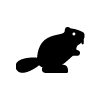
\includegraphics[width=15pt]{img/noun_Beaver_1604196}}
\newcommand{\corn}{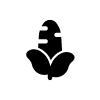
\includegraphics[width=15pt]{img/noun_Corn_2550101}}

\title{\vspace{-10pt}\Huge Site-to-Site Internet Traffic Control}
\author{
    \vspace{-20pt}
    \Large
Frank Cangialosi\footnotemark[1]\beaver,
Akshay Narayan\footnotemark[1]\beaver,
Prateesh Goyal\beaver, \\\vspace{-5pt}
Radhika Mittal\corn,
Mohammad Alizadeh\beaver,
Hari Balakrishnan\beaver
}
\affiliation{\beaver MIT CSAIL \corn UIUC}

\renewcommand{\shortauthors}{Cangialosi and Narayan, et al.}

%
\date{\vspace{-12mm}}
%
\begin{abstract}

%While multiple scheduling and queue management algorithms have been proposed in the past, very few have been implemented in today's routers and even fewer have enabled by, and used effectively, by the public network operators. 
%The Internet has been unable to enjoy the benefits of scheduling policies, due to two primary reasons: (i) network operators are unable to choose appropriate policies due to lack of visibility into individual customer’s traffic, and (ii) customers are unable to enforce their desired policies due to lack of control over queue-up links in the middle of the network. 
Internet content providers  can benefit from applying different scheduling and queue management policies to their traffic. However, they currently lack control over the queues that build up at the bottleneck links in the network to effectively enforce desired policies. To address this issue, we propose a new kind of middlebox, called \name, which brings the queues in the network under the content provider's control. \name sits at the edge of a sender's domain, and bundles together groups of flows that share a common destination domain. It does rate control for each bundle, such that the queuing induced by its traffic is moved from the bottleneck (wherever it might be in the network) to \name itself. This allows the sender to unilaterally enforce its desired scheduling policy across the bundled traffic. \name has an immediately deployable, light-weight design, which we implement in only $\sim1500$ lines of code. Our evaluation, on a variety of emulated scenarios, shows that scheduling via \name can result in up to \hb{up to is weasel wording} \an{62\%} improvement in median flow completion time compared to the status quo.

%It does 
%This works by shifting the network bottleneck from the middle of the network, where it is difficult to enforce policies, to the edge (\ie the \name), where it is easy to do so.

%Our proposed design for a \name is flexible, scalable, compatible with hardware implementations, simple (we implement it in approximately $1500$ lines of code) and can yield up to a \an{double check for more recent numbers: 62\%} improvement in median flow completion time (FCT).

% We propose a new kind of middlebox, called a \name, which manages \emph{traffic aggregates}, or a group of flows with a common origin domain and destination domain. \name can allow senders of traffic aggregates to unilaterally impose scheduling policy on component flows. This works by shifting the network bottleneck from the middle of the network, where it is difficult to enforce policies, to the edge (\ie the \name), where it is easy to do so.

% We propose a design of a \name which is flexible, scalable, compatible with hardware implementations, simple (we implement it in approximately $1500$ lines of code) and can yield up to a \an{double check for more recent numbers: 62\%} improvement in median flow completion time (FCT).
\end{abstract}

\maketitle
\setcounter{footnote}{1}
\footnotetext{Both authors contributed equally to this work.}
\renewcommand*{\thefootnote}{\arabic{footnote}}
\setcounter{footnote}{0}
\begin{sloppypar}
\section{Introduction}\label{s:intro}

This paper introduces the idea of {\em site-to-site} Internet traffic control. By ``site'', we mean a single physical location with tens to many thousands of endpoints sharing access links to rest of the Internet. Examples of sites include a company office, a coworking office building, a university campus, a single datacenter, and a point-of-presence (PoP) of a regional Internet Service Provider (ISP). 

%When a site originates traffic, the administrator of the site often has high-level objectives for their traffic, but cannot achieve those objectives today because the bottlenecks are elsewhere. 

Consider a company site with employees running thousands of concurrent applications. The administrator may wish to enforce certain traffic control policies for the company; for example, ensuring rates and priorities for Zoom sessions, de-prioritizing bulk backup traffic, prioritizing interactive web sessions, and so on. There are two issues that stand in the way: first, the bottleneck for these traffic flows may not be in the company's network, and second, the applications could all be transiting different bottlenecks. So what is the company to do?
%, and experiencing poor quality because of traffic from other sources outside the company's control. 

Cloud computing has made the second issue manageable. Because the cloud has become the prevalent method to deploy applications today, applications from different vendors often run from a small number of cloud sites (e.g., Amazon, Azure, etc.). This means that the network path used by these multiple applications serving the company's users are likely to share a common bottleneck; for example, all the applications running from Amazon's US-West datacenter, all the video sessions from a given Zoom datacenter, and so on. In this setting,  by treating the traffic between the datacenter site and the company site as a single aggregate, the company's network administrator may be able to achieve their traffic control objectives.

%e.g., ensuring that video sessions get adequate rates, de-prioritizing bulk backup traffic, prioritizing interactive web sessions, etc.

But what about the first issue? The bottleneck for all the traffic between Amazon US-West and the company may not be the site's access link or at Amazon, but elsewhere, e.g., within the company's ISP; indeed, that may be the common case~\cite{inferring-interdomain-congestion, isp-throttle-1, isp-throttle-2, isp-throttle-3}. Unfortunately, the company cannot control traffic when the queues are inside its ISP. And the ISP can't help because it does not know what the company's objectives are.\footnote{Interdomain QoS mechanisms~\cite{braden1997resource, wroclawski1997use} have not succeeded in the Internet despite years of effort.}

%a coworking space might want fairness between the traffic of resident companies to different cloud datacenters. A company may want to prioritize video conferencing traffic over other traffic (e.g., bulk backup). 

%% Example objectives
\begin{figure*}[ht!]
    \centering
    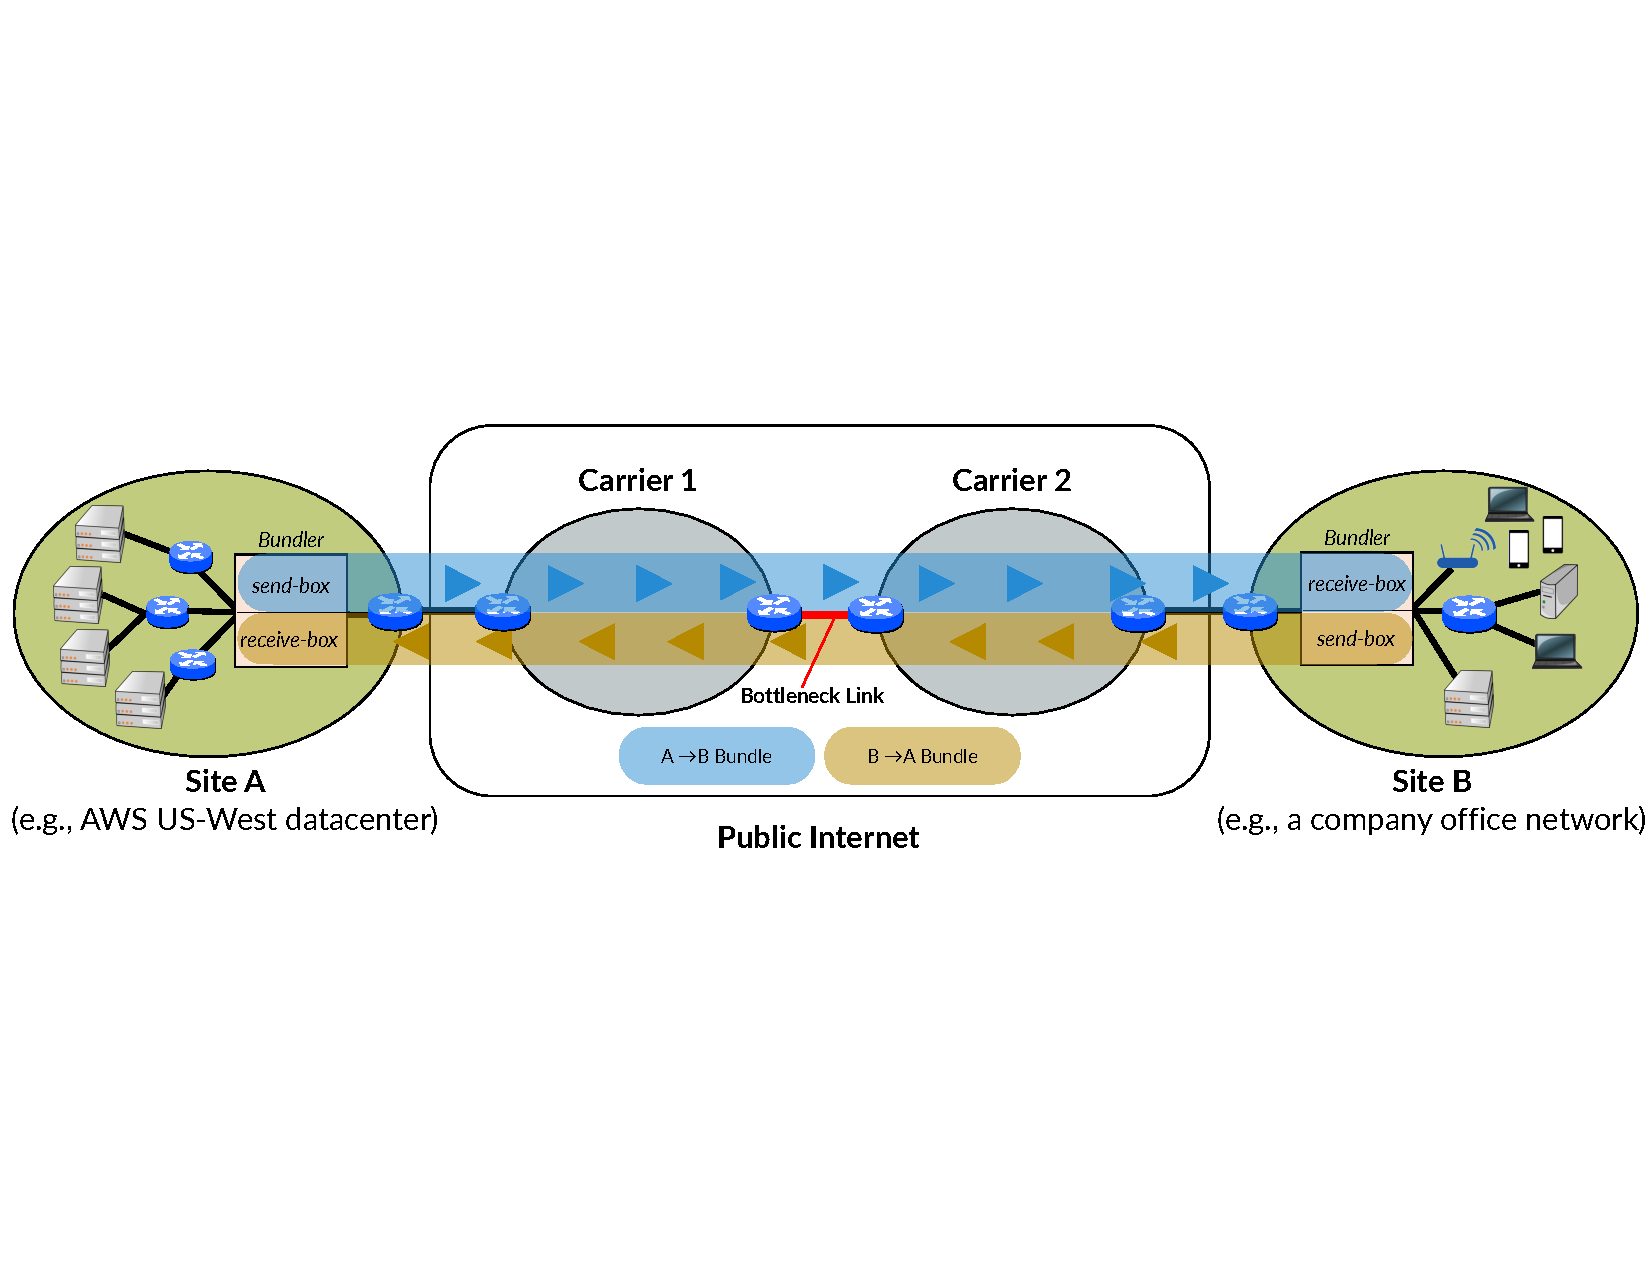
\includegraphics[width=\textwidth]{img/deployment-arch.pdf}
    \caption{An example deployment scenario for \name in sites A and B.
    Traffic between the two boxes is aggregated into a single bundle, shown as shaded boxes. The \inbox schedules the traffic within the bundle according to the policy the administrator specifies (\S\ref{s:design}).
    \an{site a and site b should be flipped}
    }
    \label{fig:deploy:arch}
\end{figure*}


We propose a system, {\em \name}, that solves this problem. \name enables flexible control of a traffic {\em bundle} between a source site and a destination site by {\em shifting} the queues that would otherwise have accumulated elsewhere to the source's site (Figure~\ref{fig:design:shift-bottleneck}) \cut{\radhika{should we instead refer to Fig 2 here?}}. It then schedules packets from this shifted queue using standard techniques~\cite{diffserv, fair-queueing, sfq, pie, CoDel, fifoplus, virtualClocks, csfq, drr, red, ecn} to reduce mean flow-completion times, ensure low packet delays, isolate classes of traffic from each other, etc.

%The most effective place to enforce a scheduling policy is where queue buildup occurs; where there is queueing, there is the opportunity to reorder packets and apply mechanisms~\cite{diffserv, fair-queueing, sfq, pie, CoDel, fifoplus, virtualClocks, csfq, drr, red, ecn} to reduce mean flow-completion times, ensure low packet delays, isolate classes of traffic from each other, etc.

%An increasing number of use cases involve sites that need to exchange large quantities of traffic on the Internet. 
%Examples include traffic between a content provider (\eg Amazon, Google, etc.) and a network with many clients (\eg an enterprise), between two different campuses of an organization, between collaborating institutes, and so on.

%The flows within such a bundle are likely to share common bottlenecks in the network connecting the two domains (as shown in F). 
The key idea in \name is a control loop between the source and destination sites to calculate the dynamic rate for the bundle. Rather than terminate end-to-end connections at the sites, we leave them intact and develop an ``inner loop'' control method between the two sites that computes this rate. The inner control loop uses a delay-based congestion control algorithm that ensures high throughput, but controls {\em self-inflicted queueing delays} at the actual bottleneck. By avoiding queues at the bottleneck, the source site can prioritize latency-sensitive applications and allocate rates according to its objectives.

By not terminating the end-to-end connections at the sites, \name{} achieves a key benefit: if the bottleneck congestion is due to other traffic not from the bundle, end-to-end algorithms naturally find their fair-share. It also simplifies the implementation because \name{} does not have to proxy TCP, QUIC, and other end-to-end protocols.

%Bundler uses a middlebox at the source site and another at the destination site to determine the time-varying rate of the path between the sites using a control loop


%\an{maybe refer to figure 1/example scenario? or cite something? as is, this seems like a point reviewers might complain about.}

 %Such links with queue build-up are often outside the control of individual content providers, which prevents them from enjoying the benefits of scheduling.
%content providers and end users have been unable to enjoy the benefits of scheduling policies. 

% ISP's cant solve problem (e.g. with CSFQ)

\if 0
ISPs, on the other hand, do control the bottleneck links in their carrier networks where different scheduling and queue management policies can be effectively enforced. 
However, ISPs neither have enough visibility into their customers' traffic to choose desired policies on their queues, nor enough incentives to enforce them\footnote{The case for private WANs is different, since they are owned by a single entity, and have, thus, been successful in exploiting the benefits of scheduling~\cite{swan, b4, bwe}. Our focus is public networks.}. Even if an ISP isolates each its customers' traffic (\eg with fair queueing~\cite{fair-queueing}), that still does not serve a customer's desire to enforce different scheduling policies within its own traffic.  
Large customers might be able to negotiate expensive deals with certain carriers to enforce specific policies~\cite{att-qos}. 
However, it might not be possible to negotiate such deals with \emph{all} carriers in the traffic's path, and content providers may wish to keep some of their policies confidential from downstream ISPs. 

\fi

%Note that simply isolating each customer (\eg with fair queueing~\cite{fair-queueing}) is not enough;  but users must still cope with self-inflicted queueing.

% introduce concept of bundles

\if 0

Meanwhile, traffic in the contemporary Internet is steadily aggregating amongst a small number of entities~\cite{fivecomps}. 
Examples include large amounts of traffic between a content provider (\eg Amazon, Google, etc.) and a network with many clients (\eg an enterprise), between two different campuses of an organization, between collaborating institutes, and so on.
We view the traffic that flows between a given sender's domain and destined for the same receiving domain, as a single, aggregate entity, that we call a \emph{bundle}.
The flows within such a bundle are likely to share common bottlenecks in the network connecting the two domains (as illustrated in Figure~\ref{fig:deploy:arch}). %\an{maybe refer to figure 1/example scenario? or cite something? as is, this seems like a point reviewers might complain about.}

% move the queues
We leverage this trend to reduce a content provider's dependence on the ISPs with respect to how its traffic is managed. In particular, we propose deploying a delay-based congestion controller at the edge of the sender's domain that controls the aggregate outgoing rate of each traffic bundle to match its bottleneck rate in the network. This effectively \emph{moves} the queues built by the traffic in the bundle from the bottleneck within the network to the sender’s domain itself, thus allowing the sender to enforce its desired traffic management policies on it. 

\fi


%Developing such an aggregate rate controller is the primary focus of our work. 

%bringing the content provider's traffic bundle(s) under its own control by \emph{moving the packet queues from the in-network bottleneck to the provider's edge}. 
%The natural question that arises is, how can the queues be ``moved''? 

%We further note that middleboxes are now prevalent in the Internet architecture~\cite{aplomb}. They are often deployed at the egress and ingress of a network domain, to ensure traffic transits them for intrusion detection, packet inspection, filtering etc. They thus provide an effective vantage point for aggregating and managing traffic. 



%Our key insight (discussed in \S\ref{s:design}) is the bundle rate control mechanism: to move the queues, we can simply use a delay-controlling congestion control algorithm. \radhika{can i chop this?}
%\an{shouldn't we keep the key insight in the intro?}

As shown in Figure~\ref{fig:deploy:arch}, \name implements its source site and destination site functions in a \emph{\inbox} and \emph{\outbox}, respectively. The \inbox of one site pairs with the \outbox of another site when sending traffic to it.\footnote{One \inbox can pair with multiple {\outbox}es and vice versa.} 
%We thus define a \emph{bundle} to be a group of flows that share the same \inbox-\outbox pair.
These two middleboxes measure congestion signals such as the round-trip time (RTT) and the rate at which packets are received, and pass these signals to a congestion control algorithm at the sendbox (\S\ref{s:design}) to dynamically compute the bundle's sending rate.
%The \inbox passes these signals to a delay-based congestion control algorithm (as described in \S\ref{s:design}) which computes appropriate sending rates for each bundle, such that the queuing induced by the bundled traffic within the network is low and is incurred at the \inbox instead, while still maintaining high utilization at the bottleneck link.
We introduce a lightweight method for the coordination between the \inbox and the \outbox that does not require any per-flow state and can be deployed in a mode that forwards packets without modification.  \name requires no changes to the end hosts or to network routers.
 
Our focus thus far has been to control traffic only within a given bundle and not across different bundles. 
Furthermore, as we will discuss in \S\ref{s:deploy}, there may be instances where \name cannot improve performance for the bundled traffic, and falls back to the status quo; \ie the performance achieved today when queues build in the network instead of the edge. For example, when traffic between the two sites traverses different paths with different levels of congestion, \name will detect this and performance will revert to the status quo.
%\cut{, but if all of these paths have the same rates, then performance will improve.\fc{<- can we cut last phrase?}}
 
In emulated scenarios (\S\ref{s:eval}), we demonstrate that \name successfully enables scheduling benefits. In particular, when configured to use Stochastic Fairness Queueing (SFQ),
\name reduces the median flow completion time (FCT) of a representative flow size distribution between 28\% to 97\% across a variety of scenarios. Furthermore, these performance benefits are within 15\% of what would be achievable if (optimal) in-network scheduling were a possibility.
In experiments over the public Internet (\S\ref{s:eval:realworld}), we find that \name reduces short-flow latencies by 57\%.

%TODO: Add evaluation highlights

\if 0
Despite these limitations, we believe that our work provides a deployable solution for enabling some of the benefits of scheduling and queue management in the Internet from the edge of the content provider's network.
 \fi
 
 \if 0
We make the following contributions:
\begin{enumerate}
    \item A light-weight, scalable, and deployable architecture that enables content providers to perform scheduling across traffic with a common destination domain. In this architecture, content providers perform congestion control over bundles of traffic with a common destination domain in order to move queueing to the content provider's edge (\S\ref{s:design}).
     \item A novel low-overhead protocol-agnostic technique for measuring signals for congestion control between the \pair, that need not make any changes to the packet headers (\S\ref{s:measurement}).
     \item A new congestion controller, synthesized from existing building blocks in congestion control (delay-control~\cite{copa}, AQM~\cite{pie}, and cross-traffic inference~\cite{nimbus} for use with traffic bundles (\S\ref{s:queue-ctl}).
     %\item The design and implementation of a \name, including a novel method of collecting congestion control information and enforcing the decisions of a rate control algorithm on traffic aggregates, which \emph{moves} the queues from the bottleneck in the network to the customer's edge.
     %\item An evaluation of the benefits of scheduling and queue management for traffic aggregates, compared to both the status quo (FIFO) and an idealized deployment where bottleneck queues deploy the desired policy.
\end{enumerate}
\fi

\section{Related Work}
\label{s:related}

%With our work sitting at the intersection of highly popular topics of scheduling, congestion control and middleboxes, one can produce a large body of past work related to each topic. However, this unique intersection of topics is also what adds significant novelty to our work. 

\Para{Traditional congestion control}
End hosts employ congestion control algorithms that aim to achieve high throughput and low delay while fairly sharing network resources with other users~\cite{Jacobson88}. 
Each connection runs such an algorithm independently to learn about the network conditions and find the best sending rate.
In \name, a \inbox uses such an algorithm to determine the aggregate's sending rate, rather than the rate of an individual connection. 
The end-hosts continue to use unmodified end-to-end congestion controllers for each connection.

\Para{Aggregating congestion information} 
% something like:
% - congestion control is xyz
% - it is typically done independently by each flow
% - however, many flows from the same sender often traverse the same bottleneck. each flow independently learning about the network is inefficient.
% - as a result, there have been multiple proposals to aggregate cc information: 1,2,3
%However, as noted in prior work, in cases where there are a large number of flows between the same sender and receiver, each flow independently learning about the network is inefficient, and it would make much more sense for them to share information.
There have been multiple proposals to aggregate congestion control information in different contexts: flows sharing the same endpoint~\cite{cm}, flows between two racks within a datacenter~\cite{rackcc}, and flows originating from a large cloud/content provider~\cite{fivecomps}. 
The goal of these approaches is to share information among the various end-to-end flows' congestion controllers, which allows them to better adapt to network conditions. 
%As traffic controllers, however, aggregate congestion control schemes cannot enforce precise traffic scheduling policies due to control overheads \fc{what does this mean?}.
\name has a different goal: to control queueing (and thus enable scheduling) from the edge of the network without interfering with the end-to-end congestion controllers of individual component flows. It is orthogonal to prior proposals on aggregate congestion control.
%\name uses aggregate congestion control in a different way (with a different goal): as a light-weight mechanism to shift the queues from the middle of the network to the edge, without interfering with the end-to-end congestion controllers of individual flows. It is orthogonal to prior proposals on aggregate congestion control.

\Para{Using a middlebox for queue management} Remote Active Queue Management (AQM)~\cite{ardelean} aims reduce VoIP traffic latency by deploying a middlebox at a site's access link that drops packets or injects ECN marks for the remaining flows in order to manipulate their end-to-end congestion control loops. It makes a core assumption that the bottleneck is the site's access link.
%, and because it relies on manipulating end-to-end congestion controllers, its component traffic must have specific characteristics, \ie those of VOIP traffic.
In contrast, \name tackles arbitrary bottleneck locations in the middle of the network. Moreover, unlike Remote AQM, \name is not restricted to a specific queue management policy for a specific traffic class.

%Remote Active Queue Management~\cite{ardelean} proposed to manipulate end-to-end congestion control loops to achieve a traffic control objective by dropping packets or injecting ECN marks. However, it makes the core assumption that the bottleneck is the site's access link, and because it relies on manipulating end-to-end congestion controllers, its component traffic must have specific characteristics, \ie those of VOIP traffic. 
%Instead, \name works with arbitrary bottleneck locations in the middle of the network and imposes an out-of-band control loop which is compatible with any component traffic (\S\ref{s:design}). 
%\radhika{not clear what remote AQM is, how its different from regular AQM, and why it is related. Lets quickly discuss} 
%\fc{not sure if we can say arbitrary -- if bottleneck is outside of the pair, bundler won't do anything. maybe better distinction is just that we target different scenarios and are thus orthogonal.}\an{clarified middle of network}

%A recent proposal~\cite{fivecomps} observes that the majority of today's traffic is owned by a few entities.
%This observation implies that there are large bundles in practice, resulting in greater scheduling opportunities within a bundle. 
%The proposal uses its observation to advocate sharing congestion information across a given domains endhosts. 
%This is orthogonal to our goal of scheduling such traffic by introducing a middlebox without modifying end hosts.

\Para{Overlay networks} \name's motivation is closer to a proposal in overlay networks, OverQoS~\cite{overqos}, which aimed to provide QoS benefits in the Internet by enforcing traffic management policies at the nodes of an already-deployed overlay network~\cite{ron}. 
\name's approach is more lightweight; instead of relying on an overlay network, \name only requires each site to deploy a middlebox, and uses a novel control loop between the middleboxes to facilitate traffic management at the sites. 
%\fc{can we also say something about not modifying traffic so its incrementally deployable?}\an{overlay networks can also claim to not modify traffic and be incrementally deployable, right}
%This simplifies the ``rendezvous'' problem, since \name initializes bundles dynamically (\S\ref{s:design}).
%In addition, \name provides a novel mechanism to \emph{move} the in-network queues, and gain the power to schedule the bundled traffic. 

%\Para{Packet scheduling} There have been some recent efforts towards enabling the benefits of packet scheduling. Most are complementary with \name and could be used as its datapath.
%For example, PIFO~\cite{pifo} is a priority queue for programmable switching chips. 

%However, not only does it require changing  in-network routers, but it also suffers from the issue of an ISP's limited visibility into the traffic to choose desired policies (and limited incentives to enforce them). 
%UPS~\cite{ups} allows different scheduling policies to be expressed from the edge via header initialization, but also requires a change to the routers.
%However, since queuing still occurs in the middle of the network, it relies on the customers targeting a common global objective, or on the network operators isolating different customers' traffic, both of which are difficult to realize. 
%\name provides a solution that does not require any cooperation from downstream networks in other organizations.

\section{Goals and Assumptions}\label{s:deploy}
\begin{figure*}[ht!]
    \centering
    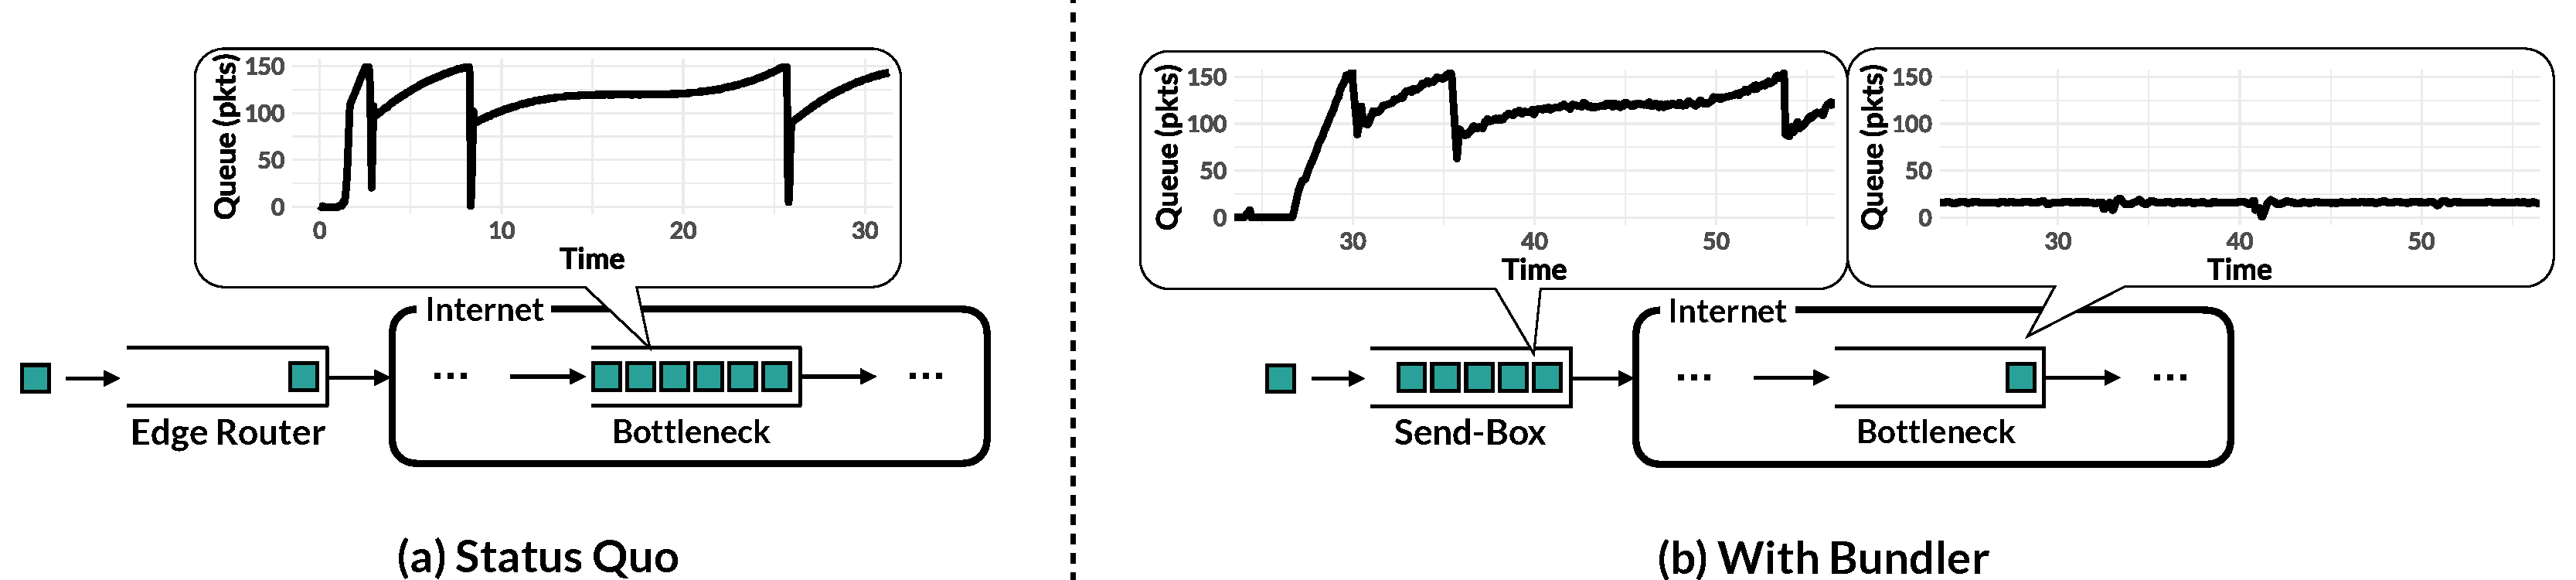
\includegraphics[width=\textwidth]{img/shift-bottleneck-combined}
    \caption{This illustrative example with a single flow shows how \name can take control of queues in the network. The plots, from measurements on an emulated path (as in \S\ref{s:eval}), show the trend in queueing delays at each queue over time. The queue where delays build up is best for scheduling decisions, since it has the most choice between packets to send next. Therefore, the \inbox \emph{shifts} the queues to itself.}\label{fig:design:shift-bottleneck}
\end{figure*}

%\fc{Would it be better to lead with some example of how theres a large amount of traffic bewteen A and B? }

%%\radhika{add more examples}
%%
%%\radhika{Add a new section on ``Requirements/Assumptions'' here that has the text below}
%%
%%\cut{
%%\Para{Amount of Aggregation} 
%%A traffic bundle, to be useful, must be \emph{heavyweight} enough to drive self-inflicted queueing in the network; these queues, once under \name's control, provide scheduling opportunities. We expect many bundles to be heavyweight in practice because a majority of Internet traffic today is owned by a few large content providers who host a wide array of services~\cite{fivecomps, labovitz}. 
%%}

Figure~\ref{fig:deploy:arch} describes \name's deployment model. 
\name aggregates traffic from Site A to Site B, and vice-versa, into two unidirectional bundles. 
In the egress path, the \inbox moves the in-network queues built by the bundled traffic to itself (illustrated in Figure~\ref{fig:design:shift-bottleneck}) (we describe the specific mechanism in \S\ref{s:design}). 
It can thus enforce desired scheduling policies across the traffic in the bundle.

Our primary goal with \name is to provide control over \emph{self-inflicted} queueing, \ie when traffic from a single bundle causes a queue to build up at the bottleneck links in the network, even without any other cross-traffic.
%cases when traffic within the same bundle should be reordered according to the site administrator's policy.
In the remainder of this section, we detail the conditions in which \name can achieve this goal. Our high-level strategy is ``do no harm''; \name detects conditions in which it cannot operate and temporarily disables itself until favorable conditions return, reverting to status-quo performance in the meantime.
%\radhika{read again after intro has been written}

\Para{Non-edge bottleneck}
Network administrators already have control over packets which queue within their site. \name is capable of taking control over queues that build up anywhere between a \pair. Thus, deploying \name at the edge of each site captures any potential build up outside of either site's control. Such congestion might occur at an inter-domain link, within either site's ISP, or, if a site is managed by a cloud provider, it could even occur within its datacenter (\eg{} at the cloud provider's rate limiter, \S\ref{s:eval:realworld}). 
% \name is thus useful for moving queues that build up due to congestion in the ``middle'' of the network (\ie \emph{anywhere} along the path between a \pair). 

There is strong evidence that such non-edge bottlenecks exist.
Dhamdhere \etal measured~\cite{inferring-interdomain-congestion} inter-domain bottlenecks such as the red bottleneck link in Figure~\ref{fig:deploy:arch}.
Similarly, Zhu \etal found~\cite{bottleneck-of-china} that non-edge bottlenecks for transnational traffic to and from China are prevalent, and moreover that in many cases, the bottleneck for this traffic is an ISP deep inside China rather than a larger provider.
An M-Lab technical report similarly found~\cite{mlab-tr} patterns of performance degradation linked to specific ISP interconnections in the middle of the network.
Finally, Jin \etal found~\cite{blameit} that for WAN traffic originating from Microsoft Azure, the ``middle'', \ie on-path ASes not including the source or destination AS, is to blame for between $40$-$50\%$ of persistent congestion incidents over a one-month period. 

\Para{External congestion} Other than self-inflicted congestion, \name must coexist with traffic from external sources.
%It can happen when a small carrier network does not have enough capacity to sustain the large volume of traffic sent by a content provider to a receiving domain, or due to explicit rate limiting commonly done by ISPs~\cite{isp-throttle-1, isp-throttle-2, isp-throttle-3}. 
%In such cases, \name can result in significant improvements in performance, as it would then have control over the entire queue. 
%In our experiments (\S\ref{s:eval}), we found this to be the case.

\vspace{2pt}
\paragraphi{Congestion due to bundled cross-traffic}
%In-network congestion can further increase in the presence of other cross-traffic (\eg when the peering link between Carrier 2 and the enterprise in Figure~\ref{fig:deploy:arch} is shared by traffic from multiple content providers' domains). 
\name continues to provide benefits when the competing flows are part of other bundles from/to other sites because the rate control algorithm at each of the other {\inbox}es would ensure that the in-network queues remain small, and different bundles compete fairly with one another. Since each \inbox manages the self-inflicted queues for its own bundles, it can apply the appropriate scheduling policy in its per-bundle queues.
%\fc{X?->}We expect this to become the common form of observed congestion as more sites deploy \name. 

\vspace{2pt}
\paragraphi{Congestion due to un-bundled cross-traffic} We now consider the scenario where the cross-traffic includes un-bundled flows. If all such \emph{un-bundled} competing flows are short-lived (up to a few MBs) or application-limited (\eg a paced video stream), the bundled traffic still sees significant performance benefits, because there are not enough packets in such short-lived flows to fill up the queues or claim a greater share of network bandwidth.
%\radhika{Likewise, \name continues to provide performance benefits in the presence long-lived rate-controlled cross-traffic (e.g. a paced video stream) that also does not fill up queues.} 
However, if the cross traffic is long lasting, and employs a loss-based congestion controller to send back-logged bulk data, it aggressively fills up all available buffer space at the bottleneck link. Naively using a delay-based congestion controller at \name against such aggressive \emph{buffer-filling} cross-traffic would severely degrade the throughput of the bundled traffic. Therefore, \name's congestion controller detects the presence of buffer-filling cross-traffic;
% to compete fairly, pushes more packets into the network. 
to compete fairly, it relinquishes most of its control (and scheduling opportunities) over the bundled traffic, while still maintaining a small queue for continued detection of cross-traffic (detailed in \S\ref{s:buffer-filling}). 
%\radhika{cut:/*} This extra queueing results in a slight latency increase that we evaluate in \S\ref{s:robust:cross}.\radhika{*/}
%However, in these cases, \name chooses to create extra queueing as described in \S\ref{s:queue-ctl} to be able to detect when the cross traffic leaves.
%Therefore, the bundle's aggregate throughput will decrease slightly due to RTT unfairness.
%We evaluate this phenomenon in \S\ref{s:robust:cross}.
%\radhika{Maybe add: ``Note that not all long-lasting flows are detected as buffer-filling (e.g. a video stream that sends paced packets does not fill buffers). A pathological buffer-filling flow is both long-lasting and comprises of a backlogged bulk transfer.}
However, such pathological buffer-filling cross traffic is rare.
%\radhika{cut:/*} To understand why, consider that cross traffic must be (a) bottlenecked at the same link as the bundle traffic and (b) long-lived enough to build persistent queues.\radhika{*/}
A recent study in CDNs~\cite{akamai-cdn-trace} and our analysis of a packet trace from an Internet backbone router~\cite{caida-dataset} reveal that the vast majority of connections are smaller than 1MB: too small to build persistent queues.\footnote{\cut{\radhika{check:} }This implies that flows \emph{within} a bundle may also be short-lived requests or paced audio/video traffic which, when aggregated by \name, can form a heavy, long-lasting bundle.} 
%\radhika{One might ask that given long-lasting flows are rare, how can \name do effective rate control. Should we add a footnote or a line that says ``Even the components of a bundle are likely to be short-lived flows (up to a few MBs) \fc{+1} and paced audio/video traffic that arrive at different times, creating a heavy long-lasting bundle on an aggregate.''} 
Our experiments on Internet paths (\S\ref{s:eval:realworld}), also did not encounter pathological buffer-filling cross traffic.  

%\radhika{Akshay, check this out.}
%We further analyze a packet trace from an Internet backbone router~\cite{caida-dataset}.
%The flow size distribution here is even more skewed: $97.6\%$ of flows are under $10$KB, and only $0.02\%$ of flows are larger than $5$MB.

\Para{Shared congestion across flows in the bundle} Bundler’s design for moving queues via aggregate congestion control assumes that the component flows within a bundle share in-network paths, and thus congestion. 
%\an{I am mentioning the traceroute measurements here:} 
To test this assumption, we used Scamper~\cite{scamper} to probe all paths to $5000$ random IPv4 addresses from each of $30$ cloud instances across the regions of public cloud providers AWS and Azure. In no cases did we find that probe packets took different AS-level paths through the network.
%\an{be careful about persistent imbalance claim}
%Of course, IP-level load balancing exists, and we detect it. 
However, we observed instances of IP-level load balancing in 26\% of IP hops. 
In pathological scenarios with \emph{persistent imbalance} in queueing between the load-balanced paths, \name cannot gather accurate measurements and perform aggregated delay-based rate control for the bundled traffic. 
Designing a new congestion control algorithm for such scenarios remains an avenue for future work.
Nonetheless, \name can detect these scenarios (\S\ref{s:queue-ctl:ecmp}) and disable its rate control in such cases, falling back to status-quo performance. 
We expect a well-implemented load balancer will work to prevent persistent imbalance from occurring; indeed, our success with using \name on real Internet paths (\S\ref{s:eval:realworld}) suggests that such pathological cases do not occur in practice.
%\radhika{cut:/*}Transient imbalance may be common. In these cases, \name's congestion controller, which uses a simple delay control law (\S\ref{s:design:whichcc}), may fluctuate its rate in response to measurements of the different queues. \name's control over the queue will thus fluctuate, but it can still provide scheduling benefits. \radhika{*/ we don't have results for this, right? readers may not get what we are saying at this point anyway} 
%\fc{did we intentionally remove the assumption about having "enough" traffic? i know it's fairly "obvious" but might be good to have at least one sentence clarifying this somewhere.} \radhika{i am fine with adding it back in. although, we might be saying something to that effect in the intro already.}
%Designing a new congestion control algorithm for this scenario remains an avenue for future work.
%Another common scenario is for the bottleneck to be at the edge of the receiving domain, which will again be shared across the bundled flows. Finally, even if an in-network load balancing mechanism splits the bundled flows across multiple congested paths with multiple in-network queues, \name would account for the aggregate network bandwidth and move all of these queues to the sender's domain. 

%(2) from the bundle's perspective, multiple paths appear as multiple queues, with some aggregate bandwidth capacity (\ie the max-flow of the network paths between the sending and receiving domains). While queueing may be unevenly distributed among the paths, the distribution of flows onto paths is currently random (\eg via ECMP). With \name, all these queues are moved to the \inbox, so it can schedule bundled flows deliberately rather than randomly.

\paragrapha{Intuition for \name's applicability}
Another way of understanding when \name is useful, which incorporates the three conditions above, is the following litmus test:
compare the queueing delay when all flows (\name's and cross-traffic) are in the network with the queueing delay when the \name’s flows are magically removed; if the latter is lower than the former, then \name can provide benefits.

\cut{
\vspace{0.05in}
\paragrapha{Takeaway} While \name must yield its scheduling ability in the face of aggressive, buffer-filling cross traffic and persistently imbalanced load balancing, in most scenarios it significantly improves performance (as we show in \S\ref{s:eval}).
This, combined with its deployment ease, makes a strong case for deploying \name. 
}

\section{Designing \name}\label{s:design}
%
\cut{
\an{maybe move to ``bundler's utility regime''/Overview/``Traffic Bundles'': 
What is the best way to take advantage of the existence of traffic bundles?
Broadly, there are two approaches: congestion control and in-network scheduling. 
Today, congestion control is a distributed concern: each end-host performs its own optimization to achieve the highest throughput and lowest latency.
Indeed, end-host rate control is a deployed method to enforce domain-wide scheduling policy in private WANs~\cite{bwe}.
On the other hand, scheduling is an in-network concern; existing proposals such as DiffServ~\cite{diffserv} observe that the network is uniquely positioned to differentiate between different flows according to some domain-wide policy.
Scheduling presents its own challenge: because the Internet is a federated system, the link with queue build-up (and thus with the opportunity to re-order packets according to a scheduling policy) will likely be outside the sending domain's purview.

\an{don't know what to say next}
}
}

Recall that in order to do scheduling, we need to move the queues from the network to the \name. 
In this section, we first describe our key insight for moving the in-network queues, and then explain our specific design choices. 
Recall that each site deploys one \name middlebox which we logically partition into sender-side (\inbox) and receiver-side (\outbox) functionality.

\subsection{Key Insight}\label{s:design:key}
We induce queuing at the \inbox by rate limiting the outgoing traffic. 
If this rate limit is made smaller than the bundle's fair share of bandwidth at the bottleneck link in the network, it will decrease throughput. 
Conversely, if the rate is too high, packets will pass through the \inbox without queueing.
Instead, the rate needs to be set such that the bottleneck link sees a small queue while remaining fully utilized (and the bundled traffic competes fairly in the presence of cross traffic). 
We make a simple, but powerful, observation: existing congestion control algorithms calculate exactly this rate~\cite{Jacobson88}. 
Therefore, running such an algorithm to set a bundle's rate would reduce its self-inflicted queue at the bottleneck, causing packets to queue at the \inbox instead, without reducing the bundle's throughput.
Note that end hosts would continue running a traditional congestion control algorithm as before (\eg Cubic~\cite{cubic}, BBR~\cite{bbr}) which is unaware of \name.
Rather, the \inbox's congestion control algorithm acts on the traffic bundle as a \emph{single unit}.

Figure~\ref{fig:design:shift-bottleneck} illustrates this concept for a single flow traversing a bottleneck link in the 
network.\footnote{Details of the emulated network setup which resulted in the illustrated queue length time-series are in \S\ref{s:eval}.}
Without \name, packets from the end hosts are queued in the network, while the queue at the edge is unoccupied. 
In contrast, a \name deployed at the edge is able to shift the queue to its \inbox.

\subsection{System Overview}\label{s:design:overview}
\begin{figure}
    \centering
    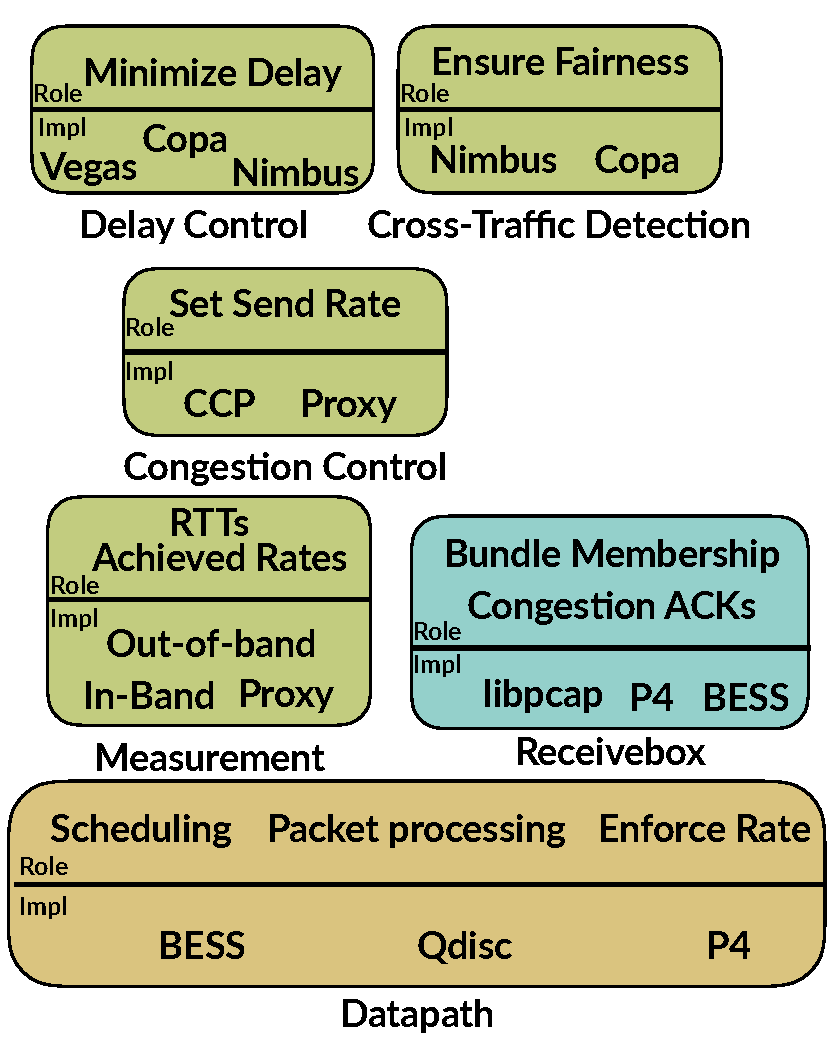
\includegraphics[width=\columnwidth]{img/arch-block-diag}
    \vspace{-40pt}
    \caption{\name comprises of six sub-systems: four (in green) implement \inbox functionality, one (in blue) implements \outbox functionality, and the datapath (orange) is shared between the two. \cut{\radhika{should we put the \name blocks inside another box called ``control plane''?}}}\label{fig:design:block-diag}
\end{figure}
%\fc{starts a bit abruptly, better lead in?}
% in order to run congestion control for an aggregation of flows, you need some way to measure the network. 
Figure~\ref{fig:design:block-diag} shows \name's sub-systems: 
(1) A congestion control module at the \inbox which implements the rate control logic and cross-traffic detection, as discussed in \S\ref{s:design:whichcc}.
(2) A mechanism for sending congestion feedback (ACKs) in the \outbox, and (3) a measurement module in the \inbox that computes congestion signals (RTT and receive rate) from the received feedback. We discuss options for implementing congestion feedback mechanism in \S\ref{s:design:twosided} and how to use that feedback in the measurement module in \S\ref{s:measurement}.
(4) A datapath for packet processing (which includes rate enforcement and packet scheduling). Any modern middlebox datapath, \eg BESS~\cite{bess}, P4~\cite{p4}, or  Linux qdiscs (as used in our prototype implementation---see \S\ref{s:impl}), is suitable. 
%\fc{should we add ecmp detection?} \radhika{can we think of it as part of measurement? let's not bring too much attention to it}
We detail the interaction between these subsystems when discussing our prototype implementation in \S\ref{s:impl}. 
%
%\an{radhika, pls check this subsection and the figure. I think it no longer requires understanding how everything works and is more of an overview?}
%\radhika{i think it looks good now! i edited it slightly -- adding more detailed sentences so that it gives a slightly more holistic overview. please check. Also, do you want to update fig 5 to make it even more consistent with this? e.g. in Fig 5, replace `Send Box' with `Measurement', `Receive box' with `Congestion ACKs', `CCP' with `Congestion Control (CCP)'? You can have the terms SendBox and ReceiveBox outside the boxes.}
%Figure~\ref{fig:design:block-diag} shows the necessary components of \name: (1) a means of determining bundle membership; (2) a rate enforcement mechanism; (3) a measurement strategy; (4) a delay-controller; and (5) a fairness-controller.
%Throughout this section we discuss design options for determining Bundle membership (\S\ref{s:design:membership}), observing feedback (\S\ref{s:design:twosided}), and congestion control (\S\ref{s:design:whichcc}): for other aspects of the design, \name is compatible with a variety of options. For example, domains can implement \name using any modern middlebox datapath, \eg P4~\cite{p4}, BESS~\cite{bess}, or as in our prototype implementation (\S\ref{s:impl}), Linux tc qdiscs.
%\radhika{maybe we can chop this subsection off -- let's discuss.}
%
In the rest of this section, we discuss our key design choices.
%Our overarching design principle is simplicity; at various points in the design, there exists a more complex approach which we discard.\fc{why? maybe just remove this?} \radhika{yes, can remove}

\cut{
\subsection{Identifying Bundle Membership}\label{s:design:membership}
\an{I think we can cut this with the site-to-site framing.}
\name must first identify which packets (or flows) are part of the same traffic bundle.
To compute and enforce correct sending rates for a traffic bundle, it is important to only bundle those flows that share the same bottleneck.
%; otherwise, \name may send a component flow at the wrong rate for its bottleneck.
This has traditionally been a difficult problem; 
Rubenstein \etal~\cite{active-sharedbottlenecks} use a ``poisson-probing'' mechanism to probabilistically identify shared bottlenecks under a limited network model, and
multipath TCP~\cite{mptcp} sidesteps it with a weighted window increase-decrease protocol.

Deploying \name boxes close to both endpoints allows us to adopt a more direct (and accurate) approach based on a \emph{two-way opt-in}.
In this approach, a site must agree to bundle traffic on both the sending and receiving sides.
The first step, of course, is to place a \name middlebox at the domain's edge.
Initially, the \inbox assumes all component traffic is unbundled.
When the \outbox observes an unbundled packet, it opts-in by sending an initialization message
\footnote{To avoid sending an initialization message for every unbundled packet, the \outbox samples the unbundled packets using the same mechanism as in \S\ref{s:measurement}.} 
(analogous to TCP's SYN) 
containing the IP prefixes it covers, addressed to the source IP of the packet
\footnote{Addressing to the source IP of the packet is not strictly necessary; domains may also advertise \inbox{}es via \eg DNS.}.
If there is no \inbox on the path, this message will be ignored.
Otherwise, a \inbox will observe this message and can opt-in by initializing a new traffic bundle corresponding to the \outbox's destination prefixes and sending a message (analogous to TCP's SYNACK) notifying the \outbox of the source IP prefixes it covers, so the \outbox can initialize a bundle corresponding to that sending domain.
Now, the \inbox and \outbox can identify packets belonging to initialized bundles by matching the corresponding IP prefixes.
Any subsequent packets the \outbox observes from that sending domain are treated as part of the bundle.

%The \outbox does one of two things for each potential epoch boundary packet:
%\begin{enumerate}
%    \item If the packet is in a known bundle, the \outbox sends a message to the corresponding \inbox.
%    \item If the packet is not in a known bundle, the \outbox sends a message to the source IP address of that packet.
%\end{enumerate}

%The \inbox receives (and intercepts) the \outbox feedback.  
%The \inbox at this time updates its flow tables to add the destination IP of the epoch boundary packet either to an existing bundle (in the case of a new flow from a previously-unseen source subnet joining a bundle) or instantiates a new bundle.
%The \inbox then sends a response containing an epoch size to use and the hash of the epoch boundary packet.
%The \outbox receives this message, initializes a byte counter for the newly discovered bundle, and remembers the \inbox IP address for future feedback. If there is no \inbox on the path, the packet will simply be ignored at its destination. 
}

\subsection{Choice of congestion control algorithm}\label{s:design:whichcc}
\name's congestion control algorithm must satisfy the following requirements: 

\paragraphi{(1) Ability to limit network queueing} \name must limit queueing in the network to move the queues to the \inbox. Therefore, congestion control algorithms which are designed to control delays, and thus queueing, are the appropriate choice. 
A loss-based congestion control algorithm which fills buffers (\eg Cubic, NewReno), for example, is not a good choice for \name, since it would build up a queue at the network bottleneck and drain queues at the \inbox.

\paragraphi{(2) Detection of buffer-filling cross-traffic} It is well known that delay-controlling schemes (\eg Vegas~\cite{vegas}) compete poorly with buffer-filling loss-based schemes~\cite{copa}.
Therefore, \name must have a mechanism to detect the presence of such competing buffer-filling flows and fall back to status quo performance, and then detect when they have left to take back its control over the network queues. 

The emergence of such detection mechanisms is recent: Copa~\cite{copa} detects whether it is able to empty the queues, and Nimbus~\cite{nimbus-arxiv} provides a more general mechanism which overlays a pattern on the sending rate and measures the cross traffic's response.
Copa is not designed for aggregate congestion control (see \S\ref{s:queue-ctl}); thus, we use the more general Nimbus mechanism.

\subsection{Congestion Feedback Mechanism}\label{s:design:twosided}
A congestion control algorithm at the \inbox would require network feedback from the receivers to measure congestion and adjust the sending rates accordingly. We discuss multiple options for obtaining this. 

%This problem presents multiple possible solutions:

\paragrapha{Passively observe in-band TCP acknowledgements}
Conventional endhost-based implementations have used TCP acknowledgements to gather congestion control measurements. A simple strategy for \name is to passively observe the receiver generated TCP acknowledgements at the \inbox. However, we discard this option as it is specific to TCP and thus incompatible with alternate protocols, \ie UDP for video streaming or QUIC's encrypted transport header~\cite{quic}.

\paragrapha{Terminate connections and proxy through TCP} With this approach, one would terminate end-host TCP connections at the \inbox and open new connections to the \outbox, allowing the \inbox to control the rate of traffic in these connections.
%This approach allows the unmodified use of existing congestion control algorithms for the TCP connection between the \inbox and the \outbox \radhika{edited, pls check}. 
%since a TCP tunnel can collect ACKs. 
This approach can improve performance by allowing end-to-end connections to ramp up their sending rates quickly. 
%\radhika{unclear} \radhika{also, wouldn't this approach have the same disadvantage as previous one?}
The primary disadvantage of this approach is that \name must take responsibility for reliable delivery of component traffic, which requires large amounts of queueing and, in the case of UDP applications, can harm application performance. 
Furthermore, proxying TCP connections introduces a new potential point of failure at \name that violates fate-sharing; if \name crashes, connections will be lost.
Finally, from a practical standpoint, to avoid head-of-line blocking this approach requires that \name open a new proxy connection for each component end-host connection, but still determine the bottleneck rate of the traffic \emph{aggregate}. While this approach may be technically feasible~\cite{cm}, it would result in high overhead.
\cut{\footnote{From an architectural standpoint this design runs counter to the end-to-end principle~\cite{e2e-principle}; it replicates endhost functionality in the network.}}
%the cycles used for opening and managing new proxy connections are better used for packet processing.
Thus, we set aside TCP proxies for the remainder of this discussion, but explore their compatibility with \name in \S\ref{s:eval:proxy}. 
%We but note that this approach is complementary with \name (see \S\ref{s:eval}).

\paragrapha{Out-of-band feedback} Having eliminated the options for using in-band feedback, we adopt an out-of-band feedback mechanism: the \outbox sends out-of-band congestion ACKs to the \inbox.
This decouples congestion signalling from traditional ACKs used for reliability and is thus indifferent to the underlying protocol (be it TCP, UDP, or QUIC).
%We detail the congestion measurement strategy and contents of congestion ACKs in \S\ref{s:measurement}.

\cut{
\begin{Appendix}
\section{Nimbus}\label{s:app:nimbus}
\begin{figure*}[ht!]
    \centering
\begin{knitrout}
\definecolor{shadecolor}{rgb}{0.969, 0.969, 0.969}\color{fgcolor}
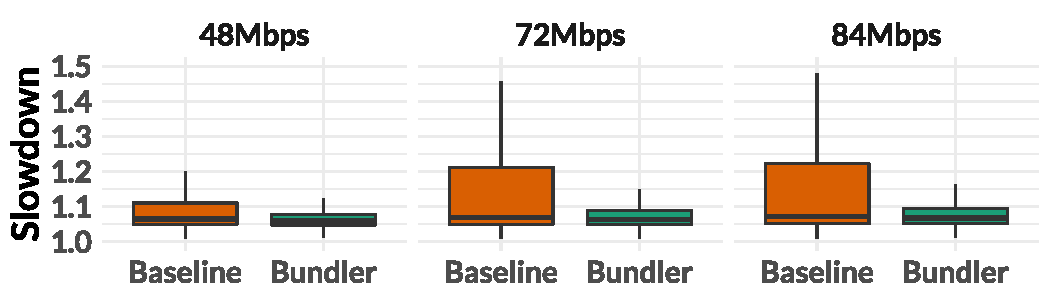
\includegraphics[width=\maxwidth]{figure/eval:offeredload-1} 

\end{knitrout}
    \caption{\name offers diminishing returns with lower amounts of offered load.}
    \label{fig:eval:offeredload}
\end{figure*}
%
%\newcommand{\highUtilTailImprove}{round(highUtilTailImprove, 0)\%\xspace}
%\newcommand{\medUtilTailImprove}{round(medUtilTailImprove, 0)\%\xspace}
%\newcommand{\lowUtilTailImprove}{round(lowUtilTailImprove, 0)\%\xspace}


We briefly summarize Nimbus~\cite{nimbus} for reference.

Nimbus's goal is to detect scenarios in which it is safe to use delay-based congestion control. 
To achieve this goal, Nimbus proposes an \emph{elasticity detector} to detect whether the cross traffic contains any \emph{elastic} flows, which react to changes in the available bandwidth on fast time-scales, \ie a couple RTTs. 
Nimbus's core observation is that the absence of such elastic cross traffic, \ie competition with only \emph{inelastic} traffic, is a sufficient (but not necessary) condition to use a delay-control algorithm.
Nimbus thus measures whether cross traffic reacts to changes in available bandwidth by pulsing its sending rate at a predetermined frequency.
If the cross traffic's rate responds to these pulses at the same frequency, Nimbus can conclude that it is elastic, because it has reacted to changes in the available bandwidth.

A natural method of measuring the cross traffic's frequency response is to compare Nimbus's pulses with the cross traffic's rate in the frequency domain.
Thus, Nimbus uses an asymmetric sinusoidal pulse (as we have noted in \S\ref{s:queue-ctl}) which has a straightforward representation in the frequency domain while maximizing the sender's ability to influence the available bandwidth.

How can Nimbus know the cross traffic's response? It develops an estimator for the cross traffic's sending rate:
\begin{equation}
    \hat{z}(t) = \mu\frac{S(t)}{R(t)} - S(t)
\end{equation}

$\hat{z}(t)i$ is the estimated cross traffic rate, $\mu$ is the estimated bottleneck bandwidth, $S(t)$ is the sending rate, and $R(t)$ is the receiving rate. 
    \name measures $R(t)$ using congestion ACKs from the \outbox and $\mu$ using the maximum receive rate as in BBR~\cite{bbr}.

Then, Nimbus searches for a peak in the neighborhood of its pulsing frequency $f_p$ to determine the elasticity metric $\eta$:

\begin{equation}
    \eta = \frac{|\text{FFT}_{\hat{z}}(f_p)|}{\text{max}_{f \in (f_p, 2f_p)} |\text{FFT}_{\hat{z}}(f)|}
\end{equation}

If $\eta$ is larger, the cross traffic is more elastic.
Nimbus then uses a hard-decision rule $\eta \ge 2$ to decide when to switch to cross-traffic competitive mode as described in \S\ref{s:queue-ctl}.

\end{Appendix}
}

\section{Measurement Strategy}\label{s:measurement}

In this section we describe how the \inbox and \outbox coordinate to compute accurate and robust
measurements of the network conditions necessary as inputs to congestion control algorithms.

Congestion control algorithms need only a small, common set of measurements~\cite{ccp-hotnets}. 
In particular, rate-based algorithms need only three measurements: 
the sending rate, receiving rate, and path round-trip time.
A significant complication is that for accurate measurements on RTT time-scales, we must calculate send and receive rates over the same set of packets~\cite{packettrain}.
This requirement drives the design of our measurement methodology.

\subsection{Determining Epoch Boundary Packets}
\label{s:measure:marking}
Consider the stream of packets $P_B$ from all flows in a bundle $B$ in the order they leave the \inbox after scheduling.
The \inbox and \outbox need to know how to divide this stream into sets 
of packets --- which we call \emph{epochs} --- over which they can calculate measurements.
For now, we make the simplifying assumption that packets arrive at the \outbox in the same order they 
left the \inbox (we address re-ordering in Section~\ref{s:measure:limitation:reorder}). \an{note about re-ordering is a little distracting and doesn't help explain approach}
This simplifies the problem into deciding, for all given packets in $P_B$, whether it is an epoch boundary packet at which the current epoch should end and the next should begin. 
Suppose for now that we wish to have a fixed epoch size of $N$ packets.
A naive approach would be to mark the boundary between epochs every $N$ packets. 
However, this strategy is brittle; a single lost packet would de-synchronize the boxes' views of the epochs. 
More generally, any strategy that requires packet-level synchronization of the \inbox and
\outbox is untenable because any coordination would race the packets themselves.

The key idea of our methodology is that we can avoid such a synchronization problem by determining the boundary of an epoch using only information contained in the packet.
Specifically, we propose the following: a packet $p$ is an epoch boundary packet if the hash 
of some subset of its header (see below) modulo the epoch size $N$ is equal to 0, that is:
$$B(p,N) \coloneqq H(p)\ \text{mod}\ N == 0$$
Thus, an epoch boundary packet will occur (in expectation) once every $N$ packets.
For $H$, we use the Fowler/Noll/Vo (FNV) hash function~\cite{fnv-hash}, a non-cryptographic fast hash function with a low collision rate. 

\paragrapha{Choosing header subset} The header subset we use must remain constant as the packet traverses the network from the \inbox to the \outbox; otherwise, they would not be able to agree on epoch boundaries. This rules out simple approaches such as hashing the entire packet header, since the TTL field will decrement between the inbox and outbox.
Even the 5-tuple of the packet may change, since the outbox may be behind a NAT.
Using TCP sequence numbers is tempting, but retransmissions may confuse RTT measurements.

We use the IP ID field, which will change every packet. This is an imperfect solution, as modern NATs may rewrite the IP ID field~\cite{ipid}.
Ultimately, the appropriate field to use will depend on the specific deployment of \name.

\subsection{Computing Measurements}
\label{s:measure:compute}
\newcommand{\pone}{$p_{prev}$}
\newcommand{\hpone}{$h(p_{prev})$}
\newcommand{\sone}{$s_{prev}$}
\newcommand{\rone}{$r_{prev}$}
\newcommand{\ptwo}{$p_{curr}$}
\newcommand{\hptwo}{$h(p_{curr})$}
\newcommand{\stwo}{$s_{curr}$}
\newcommand{\rtwo}{$r_{curr}$}
\newcommand{\atwo}{$a_{curr}$}
\newcommand{\sentone}{$sent_{prev}$}
\newcommand{\recvdone}{$rcvd_{prev}$}
\newcommand{\senttwo}{$sent_{curr}$}
\newcommand{\recvdtwo}{$rcvd_{curr}$}


\begin{figure}
    \centering
    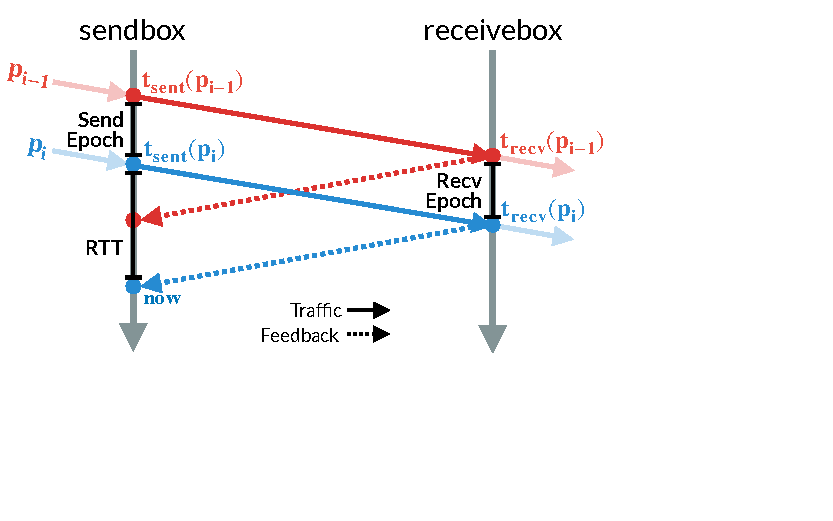
\includegraphics[width=\columnwidth]{img/rate-calculation}
    \caption{Example of epoch-based measurement calculation. Time moves from top to bottom.
    Packets from flows in a bundle
    pass through the \inbox and \outbox middleboxes on the way to their destination. When 
    the inbox observes a packet header matching the boundary condition, it records it. When
    the \outbox observes such a packet, it sends an out-of-band feedback message back to
    the \inbox, which allows it to calculate the RTT and epochs.}\label{fig:ratecalc}
\end{figure}

Given this method of marking epochs, we can now construct the procedure for computing measurements.

For a given bundle, the \inbox runs the aforementioned function on each packet $p$. Each time
the function returns true, the \inbox updates an epoch data structure that records the packet hash,
which we will call \hptwo\ for the current epoch, 
along with the current time \stwo\ and the \emph{cumulative} number of bytes sent so far, \senttwo. This structure
is sorted by the time the packet was sent, \stwo, but is indexable by the packet hash.

The \outbox runs the same function. Each time it observes a boundary packet, 
it immediately sends a feedback message to the \inbox containing the same information:
the packet hash \hptwo, the time at which it received the packet, \rtwo, and the cumulative number of bytes
\emph{received} up until that point. When the \inbox receives this feedback message at time \atwo, it looks up the
packet hash \hptwo\ in the epoch data structure, which represents the end of the current epoch,
along with the earliest boundary packet still in the data structure, \hpone\ which represents the start
of the current epoch. It now has all of the information necessary to calculate one sample of the following:
\begin{subequations}
    \begin{align}
        RTT &= &now - s_2 \\
        send\_epoch\_duration &= &s_2 - s_1\\
        recv\_epoch\_duration &= &r_2 - r_1\\
        bytes\_sent\_in\_epoch &= &bytes\_sent\ at\ s_2 &\ - \\
                                    &&bytes\_sent\ at\ s_1&\notag\\
        bytes\_rcvd\_in\_epoch &= &bytes\_rcvd\ at\ r_2 &\ - \\
                                &&bytes\_rcvd\ at\ r_1\notag\\
        send\_rate &= &\frac{bytes\_sent\_in\_epoch}{send\_epoch\_duration}\\
        recv\_rate &= &\frac{bytes\_rcvd\_in\_epoch}{recv\_epoch\_duration}
    \end{align}
\end{subequations}
%(Note $bytes\_rcvd\_in\_epoch$ can also be interpreted as the number of bytes
%acknowledged for that epoch, which is a common signal used by many conestion
%control algorithms.)
Finally, it clears all marked packets preceding \ptwo\ leaving \ptwo\
to be the start of the next epoch.

\subsection{Fault Tolerance}
\label{s:measure:loss}
\paragrapha{Packet loss} This method is robust to the loss of boundary packets between the \inbox and \outbox.
Suppose the \inbox sees boundary packets $p_1, p_2, p_3$, but $p_2$ is lost after passing through
the \inbox so the \inbox only receives feedback for $p_1$ and $p_3$. Upon receiving $p_1$, 
the \inbox will truncate its data structure up until $p_1$. Upon receiving $p_3$, the \inbox 
looks up the oldest remaining boundary packet, $p_1$, and considers that the beginning of the epoch.
As a result, the epoch is longer than expected, but no measurements are lost or corrupted. 
The same argument applies to the loss of feedback messages. 
Importantly, \inbox calculates both the send and receive epoch based on information
from the \outbox rather than attempting to reach consensus on individual epoch boundaries with the \outbox. 

\paragrapha{Crashes \an{need better heading}} Existing work~\cite{ftmb} has studied how to design stateful middleboxes to be fault-tolerant with acceptable performance overheads. 
However, state-persistence is largely unnecessary for \name.
\name only stores network conditions, which it can re-learn within a few RTTs, and bundle membership flow tables, which it can re-discover as we describe in~\S\ref{s:impl:discovery}. 

\subsection{Choosing The Epoch Size}
\label{s:measure:epoch}
How do we choose the number of packets that should be in each epoch?
In 3.1, we assumed a fixed epoch size of $N$ packets.
However, in practice, the epoch must be a function of the sending rate.
If the epoch size is too small relative to the rate,
the epochs will be easily influenced by bursts and thus the measurements will be highly variable
and not useful.
If the epoch size is too large relative to the rate, the congestion control algorithm will not
receive feedback frequently enough to respond promptly to changing network conditions. 
As shown in prior work, congestion control algorithms can behave properly even if their
signals are only updated roughly once per RTT~\cite{ccp-hotnets}.
Setting the epoch size equal to our estimate of the number of packets currently inflight 
(our current sending rate multipled by our current esimate of the RTT) will yield roughly
one epoch and thus a new set of measurements per RTT.

Since the rate and thus the number of inflight packets is continuously changing over time,
we need to continually update the epoch size. Rather than using exactly the number of inflight
bytes, we round the value down to the nearest power of two so that the new epoch size is
always a multiple of the old one and thus will be compatible. 

For examaple, \fc{is an example necessary?}
if the inbox is marking every 256 packets
and the \outbox is marking every 512 packets, 
the inbox is just marking a super set of the \outbox packets, 
so it is effectively equivalent to them both marking every 512 packets.

\fc{Add explanation of windows}.
    
\subsection{Microbenchmarks}
\label{s:measure:microbench}
    \begin{figure}
    \centering
\begin{knitrout}
\definecolor{shadecolor}{rgb}{0.969, 0.969, 0.969}\color{fgcolor}
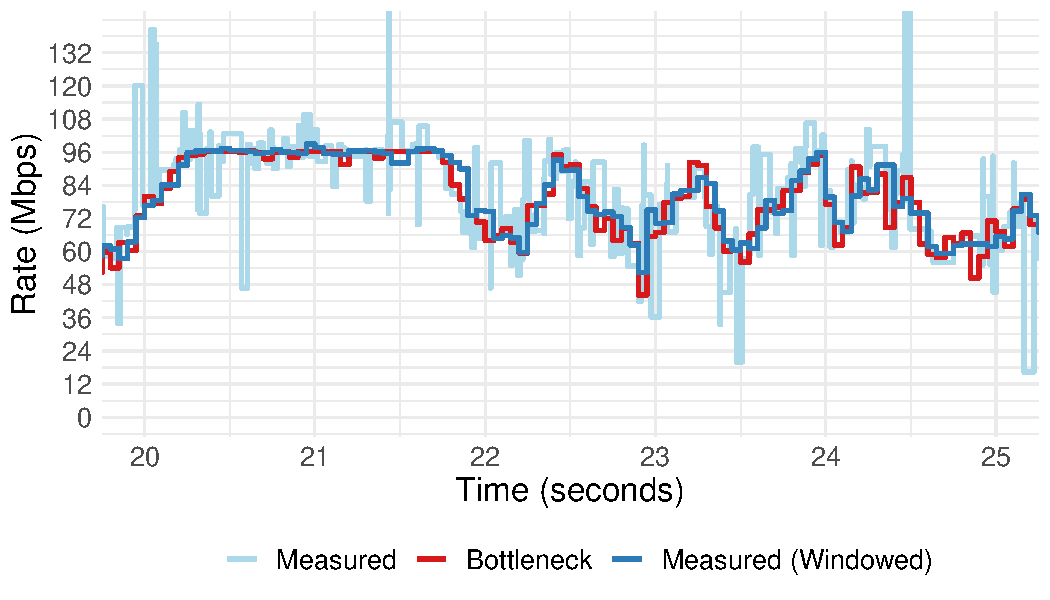
\includegraphics[width=\maxwidth]{figure/micro:time-1} 

\end{knitrout}
    \caption{\name's estimate of the receive rate compared to the actual rate leaving the bottleneck over a five second trace. 
    \name's raw estimate of the rate hovers around the true value, but is noisy. Averaging over a window of previous epochs
    yields a much smoother estimate that closely matches the true value.}
    \label{fig:micro:time}
\end{figure}

    \begin{figure}
    \centering
\begin{knitrout}
\definecolor{shadecolor}{rgb}{0.969, 0.969, 0.969}\color{fgcolor}
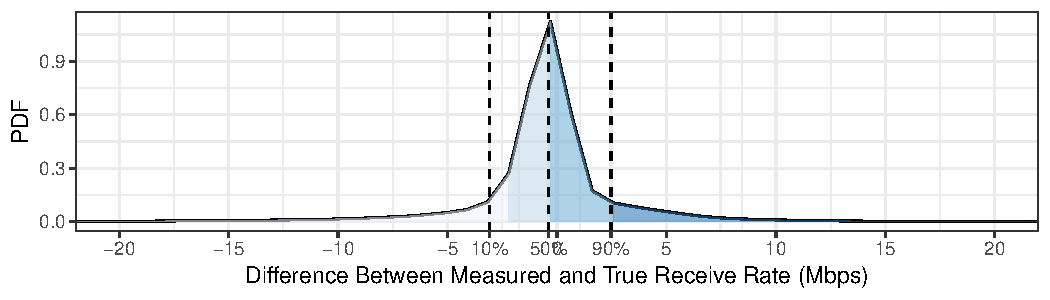
\includegraphics[width=\maxwidth]{figure/micro:thru-1} 

\end{knitrout}
    \caption{Distribution of the difference between \name's smoothed estimate of the receive rate and 
    the true bottleneck rate at each time point across all experiments. In most cases, the difference
    is negligble.}
    \label{fig:micro:thru}
\end{figure}

    \begin{figure}
    \centering
\begin{knitrout}
\definecolor{shadecolor}{rgb}{0.969, 0.969, 0.969}\color{fgcolor}
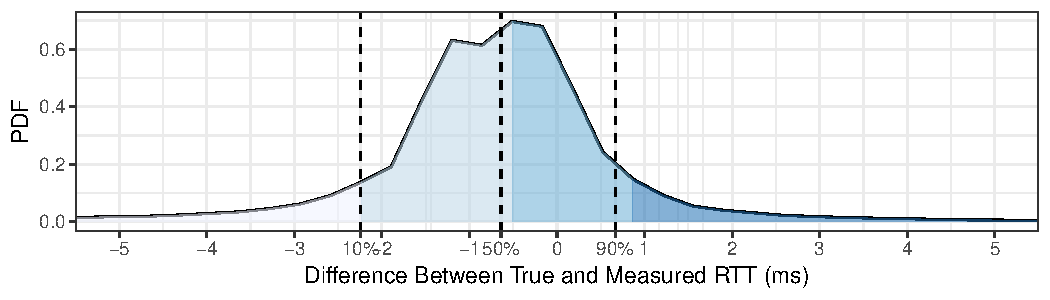
\includegraphics[width=\maxwidth]{figure/micro:delay-1} 

\end{knitrout}
    \caption{Distribution of the difference between \name's smoothed estimate of the RTT and 
    the true RTT (based on the queueing delay at the bottleneck router) at each time point across all experiments. In most cases, the difference
    is negligble.}
    \label{fig:micro:delay}
\end{figure}

    In this section we explore how well our measurements match the actual network conditions. 

    First, we consider our estimate of the receive rate (via Equation 1g). In Figure~\ref{fig:micro:time}
    we compare our esimate of the receive rate (``Measured'') to the actual rate of packets 
    leaving the bottleneck over a five second segment from one run in our evaluation (\fc{expand}).
    Here we demonstrate the necessity of a window to smooth out the estimation.

    In Figure~\ref{fig:micro:thru}, we compute the difference between our smoothed estimate of the receive rate 
    and the bottleneck rate at each time step and plot the distribution of this difference across
    all of the traces in our evaluation. 80\% of the time our estimate is within 3Mbps of the 
    actual rate.

    In Figure~\ref{fig:micro:delay}, we compute the difference between our estimate of the RTT between
    the \inbox and \outbox and the actual RTT at each time stpe and plot the distribution again
    across all of the traces in our evaluation. 80\% of the time we are within 2ms of the actual RTT.
    
\subsection{Limitations}
\subsubsection{Re-Ordering}
\label{s:measure:limitation:reorder}
Earlier we ignored re-ordering of packets between the \inbox and \outbox. However, if packets
are re-ordered, the \inbox and \outbox will observe a different view of the same epoch.
For example, consider packets numbered 1 to 20, where 10 is a boundary packet. The \inbox observes
10 packets in each epoch: [1,10] in epoch 1 and [11,20] in epoch 2. 
However, suppose packet 7 is delayed and arrives after packet 10. The \outbox will observe 9
packets in epoch 1 and 11 packets in epoch 2. 
Spurious re-ordering can be compensated by using an EWMA across epochs rather than the raw values
calculated at each epoch. If there is persitent re-ordering, it may be necessary to add a constant 
value to either the send or receive rate to compensate.

\subsubsection{Suitable Algorithms}
\label{s:measure:limitation:algs}
The set of measurements we obtain are sufficient for most rate-based algorithms, but may not be 
suitable for traditional window-based algorithms which require low-level metrics such as 
the number of inflight packets or number of packets lost. Although it should be possible
to compute these from the measurements we already collect in an ideal scenario, they would easily
break in the presence of network anomilies such as re-ordering. Thus, we leave the development
of robust signals for window-based algorithms to fuure work. 
Thus, \name currently operates best with rate-based algorithms such as BBR, Nimbus, or Copa~\cite{bbr,nimbus,copa}.


\subsection{Implications of \name's Design}

Our design choices result in an architecture where \name's inner rate control loop can be implemented entirely the ``control plane'' of the \inbox and the \outbox, which passively observes the packets traversing the datapath of the middleboxes, without modifying them. This results in a truly transparent system, that is light-weight, has low overhead, preserves fate-sharing, and in no way interferes with the end-to-end controllers of individual flows. The only datapath action that \name performs is the enforcement of the desired scheduling and queue management policies at the \inbox. 
%\radhika{added this subsection, since i think we weren't emphasizing on this enough. feel free to cut if running out of space.}

%\section{Coping with Cross Traffic}
\section{\cut{Handling }Unfavorable Conditions}\label{s:queue-ctl}

Recall from \S\ref{s:deploy} that \name can reliably shift queue build up from the bottleneck to itself when, (a) the cross-traffic is not buffer-filling, and (b) all of its component traffic shares the same bottleneck in the network.
In practice, either of these conditions may break. 
%not always hold on the real Internet, and they may change over time.
In this section, we describe how \name can re-use the same measurements from \S\ref{s:measurement} to detect when these conditions do not hold. In such cases, \name (temporarily) disables its rate limiting (falling back to status-quo performance) until favorable conditions arise again. 
%Thus, even in the worst case \name will not degrade performance (relative to the status quo without \name).
% simply degrades to status quo performance.
% Of course, in real Internet conditions, there may be scenarios where these conditions do not hold.
% In these cases, \name gracefully degrades to status quo performance. 

\subsection{Buffer-Filling Cross Traffic}
\label{s:buffer-filling}

%%%%%%%%%%%%%%%%%%%%%%%%%%%%%%%%%

% As described in \S\ref{4.3}, \name uses a delay-based congestion control algorithm to control queues in the middle of the network. 
It is well known that delay-based congestion control algorithms (as \name uses) lose throughput when competing with buffer-filling algorithms~\cite{copa, nimbus-arxiv}. 
To prevent this, \name utilizes prior work, Nimbus~\cite{nimbus-arxiv}, which provides a mechanism for detecting the presence of buffer-filling\footnote{In particular, Nimbus detects ``elastic'' cross-traffic~\cite{nimbus-arxiv}, a superset of buffer-filling traffic. \cite{nimbus-arxiv} provides an explanation of this distinction
and a detailed evaluation of Nimbus' accuracy of detecting elastic cross traffic and speed of switching between the two modes, using both emulated and real-world experiments. \name{}'s use of Nimbus does not impact its accuracy or speed of switching.} 
cross traffic, and proposes temporarily switching to a buffer-filling scheme to compete fairly whenever such cross traffic is present.
At a high-level, the detection mechanism works as follows: given a desired sending rate $r(t)$ (from an underlying congestion control algorithm), Nimbus superimposes an asymmetric sinusoid onto $r(t)$ to determine the sending rate. Then, it monitors the measured send and receive rate, estimates the cross-traffic's rate, and monitors the cross traffic's rate in the frequency domain. The sinusoidal variations in the sending rate will be visible in the cross-traffic's rate only if buffer-filling cross traffic is sharing the same bottleneck queue. 

What exactly should the \inbox do when it detects buffer-filling traffic? Using a buffer-filling scheme for the bundle as in Nimbus would be fraught: since a bundle is comprised of many individual flows, the \inbox would need to know the number of flows in the bundle to know how aggressively it should compete in order to receive its fair share (as in the status quo)~\cite{multcp}. 
This number may vary significantly over time and would be difficult to measure, especially on high-performance datapaths~\cite{heavy-hitters}.

Instead, we propose a simpler solution.
Since each connection in a bundle is already employing its own congestion controller, \name{} can simply \emph{let the traffic pass}, \ie{} increase the pacing rate at the \inbox to stop controlling queues.
Then, the end-host congestion control loops will naturally compete fairly with the buffer-filling cross traffic, just as they would without \name{}.

However, letting the traffic pass creates a new challenge. 
To determine when it is safe to resume delay-control while in the traffic-passing mode, Nimbus requires a superimposed pulse in both modes. If we naively let the traffic pass, the \inbox queue would never build. As a result, there would not be sufficient packets in the queue to perform the rate increase for the up-pulse. 
Without the up-pulse, once the \inbox{} switched to the buffer-filling mode, it would not be able to gather sufficient information to switch back to delay-control mode once the buffer-filling cross traffic subsided.

%\paragrapha{Active Probing}
% This brings us to the next natural question: how can the \inbox know when it is safe to resume delay-control (and scheduling) after disabling it?
%It is important to distinguish between \emph{self-inflicted} queueing delay and queueing delay due to cross traffic.
%When the queueing delay is purely self-inflicted, it is safe to resume control over the queues at the \inbox.
% One approach is to send passive probes along the network to detect the presence/absence of queuing. However, such passive measurements cannot distinguish between the self-inflicted queuing due to \name's traffic and the queuing due to cross-traffic. If the bottleneck queue is entirely self-inflicted, it is safe (and desirable) to resume delay-control and scheduling.
%Passive probing is insufficient to determine this state, since passive measurements of the bottleneck will be identical in the case of self-inflicted queueing and queueing driven by cross traffic.
% Therefore, it is important to \emph{actively probe}, that is, change the rate of bundled traffic and observe the response of the cross traffic. 
% This is exactly what the Nimbus mechanism does.
% At a high level,
% TODO: r(t) is the desired sending rate, A sint is super-imposed on top
% r(t) is the rate you are trying 
% something calculates r(t), calculate based on sending and receiving rate, using e.g. basic delay rule  
% now we are trying to deicde, when we want to let the pas
% we are trying to figure out the change to r(t) from the basic delay rule
% if its too large you'll converge too quickly and cant superimpose sinusoid on top of it
% given a desired sending rate $r(t)$, Nimbus superimposes an asymmetric sinusoid on top of $r(t)$, and measures the cross traffic's response in the frequency domain.
% Nimbus sinusoidally varies the sending rate $r(t) = A sin(\frac{4\pi{}t}{T})$ during the up-pulse, where $A$ is the pulse amplitude (set to one-fourth of the estimated bottleneck bandwidth) and $T$ is the pulse duration, and measures the cross traffic's response in the frequency domain.
% The \inbox can use the Nimbus algorithm to detect when to relinquish control over the queue by interposing this sending pattern over the delay-controller's rate decisions.
% However, if the \inbox entirely drains its queues into the network, it will no longer be possible for Nimbus to overlay pulses onto the traffic pattern, and it will be unable to determine the nature of the cross traffic.
% Practically, this would mean that once \inbox switches to compete with cross traffic, it would never gain the information necessary to switch back.

To support the Nimbus pulses while also letting the traffic pass,
the \inbox must maintain sufficient queueing for the up-pulse,
\ie the area under the up-pulse curve: 
$A \int_0^{\frac{T}{4}} \sin(\frac{4\pi{}t}{T}) dt = \frac{AT}{2\pi}$.
From Nimbus, we use $T = 0.2$ seconds and $A =$ one-fourth the bottleneck bandwidth. Then, by Little's law, the amount of extra queueing necessary is equivalent to
$\frac{T}{8\pi}$, or $8$ms. % We call this the target queueing delay, or $q_T$. 
We thus configure the \inbox to maintain a target queueing delay of $q_T = 10$ms (the additional $2$ms is a cushion against input variance).
Because bundled connections will experience this queueing in addition to other queueing in the network, 
most traditional congestion control algorithms (\eg Cubic) will observe RTT inflation. 
In \S\ref{s:robust:cross} we show that this effect is not large; \name still achieves performance comparable to the status quo. Nevertheless, it is desirable to be as close to $q_T$ as possible. 

Thus, to achieve the target queueing delay $q_T$
we use a PI controller at the \inbox which determines how the base sending rate $r(t)$ should be updated:
$\dot{r}(t) = \alpha (q(t) - q_T) + \beta (\dot{q}(t))$, where $\dot{r}(t)$ is the update to $r(t)$ before imposing the Nimbus pulse, $q(t)$ is the current queue size at the \inbox in milliseconds, and $\alpha$ and $\beta$ are both positive.
If $q(t) > q_T$, the first term will be positive and the rate will increase, which will drain the queue. Similarly, if the queue size is growing, the second term will be positive and the queue will grow. 
Setting $\alpha$ and $\beta$ controls a tradeoff: with larger values the controller will approach the target queueing delay faster, but if they are too large the controller's variations will dominate the Nimbus pulse. 
If they are too small, it will take too long to reach the target delay. 
We found that $\alpha=10$ and $\beta = 10$ work well for the scenarios in our evaluation (\S\ref{s:eval} and \S\ref{s:eval:realworld}).

% This problem is similar to the role of the PIE AQM mechanism~\cite{pie}, which also seeks to maintain a queueing delay target.
% Correspondingly, we design a PI controller at the \inbox as part of the fairness control module. 
% It overlays a rate $r$ corresponding to , where $q$ is the queue size and $q_T$ is the target queue size computed above.
% We pick $\alpha = 10$ and $\beta = 10$ by solving for a convergence time of one RTT (Appendix~\ref{app:derive-ab}).
% as per \S\ref{s:qctl:pi}.

\subsection{Imbalanced Multipathing}\label{s:queue-ctl:ecmp}
Since a \bundle contains many component connections, a load balancer may send them along different paths. If the load along different paths is well-balanced, \name will accurately treat a load-balanced bottleneck link as a single link whose rate is the sum of the rates of each sub-link. However, when the load along different paths is imbalanced, the series of measurements \name collects will be a random sampling of the different paths, which would confuse the delay-control algorithm and cause it to perform poorly. Fortunately, such cases are straight-forward to detect with our measurement technique. 
More specifically, load imbalance will result in many epoch measure packets arriving out-of-order at the \outbox (whenever epoch packet $i$ happens to traverse a path with a larger delay than epoch packet $i+1$), and consequently, out-of-order ``congestion ACKs'' at the \inbox.  Figure~\ref{fig:queue-ctl:ecmp:motivation} demonstrates this in an emulated imbalance scenario. 

Therefore, we use the fraction of epoch measurement packets that arrive out-of-order as an indicator of load imbalance due to multipathing.
If this number is small, the links are roughly balanced and \name will operate as expected.
If it is large, it indicates load imbalance, in which case \name's rate control may not work well. 
%While we believe that it is possible to design a rate controller that distinguishes RTT samples from different paths, and computes appropriate aggregate rates, we leave this for future research, and instead adopt a simpler
%the delay controller will make erratic adjustments as it briefly observes high RTTs, and may lose throughput as a result.
In \S\ref{s:eval:ecmp}, we experimentally determine an out-of-order fraction of 5\% to be a good threshold indicating whether or not the links are balanced: all single-path scenarios resulted in an order of magnitude fewer out-of-order packets, and all multi-path scenarios resulted in an order of magnitude greater.

% Therefore, if the reordering level is above 5\%, we disable rate control and revert to status quo performance. We evaluate this approach (and justify our chosen threshold) in \S\ref{s:eval:ecmp}.
%In this case, the measurement sub-system (\S\ref{s:measurement}) would report erratic measurements corresponding in turn to each of the possible paths.
% To see why, consider that \name's epoch-based rate measurements do not distinguish the path the packets take, and instead consider only the number of packets sent and received in an epoch.
% Thus, \name will accurately measure a load-balanced bottleneck link as a single link with the aggregate rate of each sub-link.
% However, for RTT measurements, the link with the lowest RTT will be over-sampled because the first epoch feedback packet to arrive will be from this link.
% So, \name will not detect building queues in other links.
% In most cases, this is not fatal: the delay controller might yield too much queue to the bottleneck, causing \name to miss out on performance improvements.
% We leave the design of a delay controller that does not over-react to conflicting measurements, and thus further optimizes traffic-control ability, to future work.

%In extreme cases, there may be persistent imbalance in the level of queueing. 
\begin{figure}
    \centering
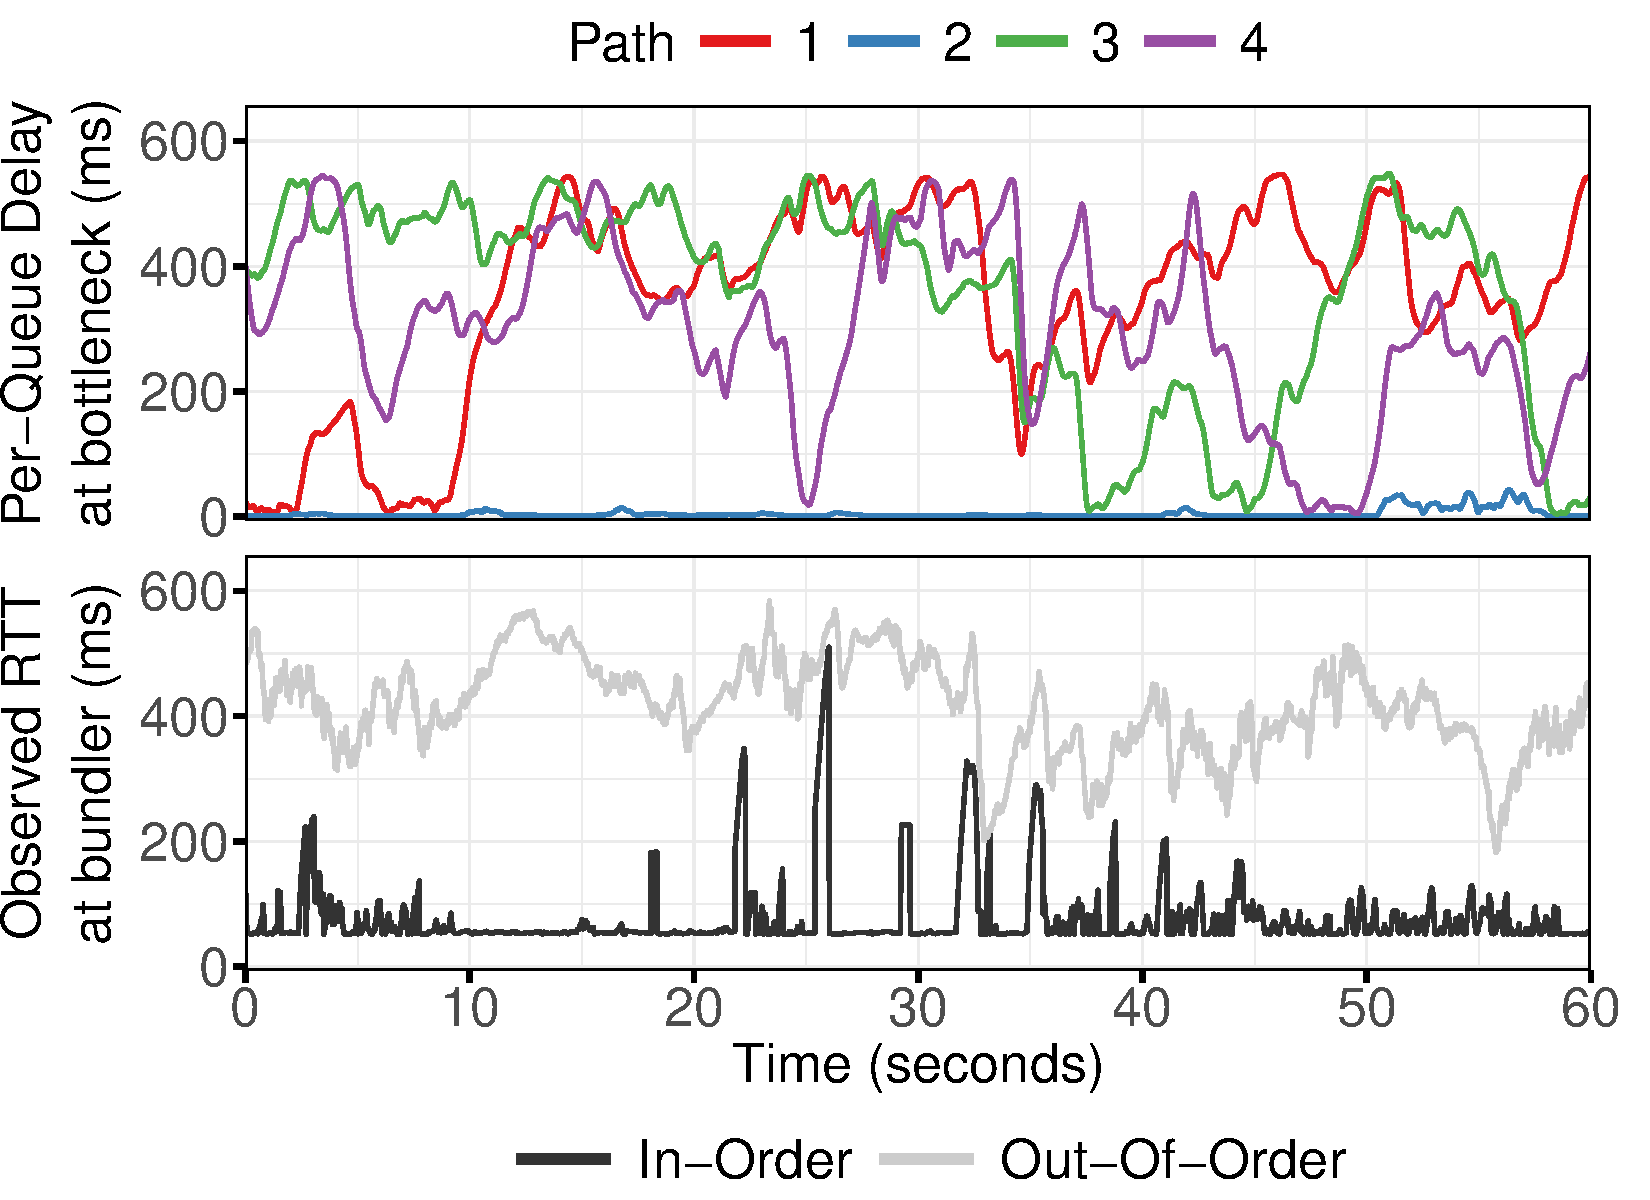
\includegraphics[width=\maxwidth]{figure/ecmp_delay.pdf} 
\vspace{2pt}
\caption{(Top) True delay for all packets of \name's component flows based on which of 4 load-balanced paths they traversed (unknown to \name). (Bottom) Delay measurements observed by Bundler, colored based on whether they were derived from an in-order or out-of-order epoch packet. Bundler's measurements cannot distinguish how many paths there are, but the relative number of out-of-order measurements is enough to clearly indicate the presence of multiple RTT-imbalanced paths.}
\label{fig:queue-ctl:ecmp:motivation}
\end{figure}


\section{Implementation}\label{s:impl}
\name boxes can be implemented as described below (although the specific implementations could vary across deployments).

\Para{\capinbox} It comprises of a \emph{data plane} and a \emph{control plane}. The data plane is responsible for (i) packet forwarding, (ii) tracking the number of sent bytes, (iii) identifying and reporting the epoch boundary packets to the control plane, (iv) enforcing a sending rate (computed by the control plane) on a bundle, and (iv) enforcing the desired scheduling policies for a bundle. 
It can implemented in software~\cite{bess, click, netbricks, tc}, or in programmable hardware~\cite{p4}. 
The control plane, implemented in software, is responsible for (i) measuring congestion signals using the information provided by the data plane along with the feedback from the \outbox, (ii) computing and communicating epoch sizes, and (iii) running the congestion control algorithm for each bundle to compute appropriate sending rates based on the measured congestion signals.

\Para{\capoutbox} It (i) tracks the number of received bytes, (ii) receives and updates epoch size values, (iii) identifies epoch boundary packets and sends feedback message to the \inbox up on receiving one. Similar to \inbox's data plane, it can also be implemented using either software or hardware.

\subsection{Prototype}\label{s:impl:prototype}

We now describe our prototype implementation of \name.

\Para{\capinbox data plane} We implement it using Linux \texttt{tc}~\cite{tc}.
We patch the TBF queueing discipline (qdisc)~\cite{tbf} to detect epoch boundary packets and to report them to the control plane using a netlink socket. 
We use the FNV hash function~\cite{fnv-hash}, a non-cryptographic fast hash function with a low collision rate, to compute the packet header hash for identifying epoch boundaries.
This hash function, comprising 4 integer multiplications, is the only additional per-packet work the data plane must perform to support \name; in our experiments, it had negligible CPU overhead.

We patch TBF's \texttt{inner\_qdisc} to support any qdisc-based traffic controller.
\cut{SFQ~\cite{sfq}, FQ-CoDel~\cite{fq-codel} and strict prioritization, in addition to the default FIFO. }
By default, TBF instantaneously re-fills the token bucket when the rate is updated; we disable this feature to avoid rate fluctuations caused by our frequent rate updates. 
Our patch to the TBF qdisc comprises $112$ lines of C.

\Para{\capinbox control plane} We implement it to run in user-space in $1365$ lines of Rust.
We use CCP~\cite{ccp} to run different congestion control algorithms (described next). 
CCP is a platform for expressing congestion control algorithms in an asynchronous format, which makes it a natural choice for our epoch-based measurement architecture. 
The control plane uses \texttt{libccp}~\cite{ccp} to interface with the congestion control algorithm, and  \texttt{libnl} to communicate with the qdisc.

\Para{Congestion control algorithms} We use existing implementations of congestion control algorithms (namely, Nimbus~\cite{nimbus-arxiv}, Copa~\cite{copa} and BBR~\cite{bbr}) on CCP to compute sending rates at the \inbox.  If the algorithm uses a congestion window, the \inbox computes an effective rate of $\frac{\text{CWND}}{\text{RTT}}$ and sets it at the qdisc. 
We validated that our implementation of these congestion control schemes at the \inbox closely follows their implementation at an endhost.

\cut{
\Para{\capoutbox} We implement it using \texttt{libpcap} in $236$ lines of Rust.
}

\subsection{\name Event Loop}\label{s:impl:loop}
Figure~\ref{fig:bundler} provides an overview of how our \name implementation operates on an already-established bundle. 

(1) In the datapath, packets arrive at the \inbox qdisc.
(2) The qdisc determines whether a packet matches the epoch boundary condition (\S\ref{s:measurement}). 
If so, it sends a netlink message to the control plane process running in user-space, and then forwards the packet normally (note the datapath does not send packets to user-space). 
(3) The \outbox observes the same epoch boundary packet via \texttt{libpcap}.
(4) It sends an out-of-band UDP message to the \inbox that contains the hash of the packet and its current state. 
(5) The \inbox receives the UDP message, and uses it to calculate the epochs and measurements as described 
in \S\ref{s:measurement}. 
(6) Asynchronously, the \inbox control plane invokes the congestion control algorithm every $10$ms~\cite{ccp}
via \texttt{libccp},
(7) The \inbox control plane communicates the rate, if updated, to the qdisc
using \texttt{libnl}. 
Finally (8), if the \inbox changes the desired epoch length based on new measurements, it communicates this to the \outbox, also out-of-band.

\section{Evaluation}\label{s:eval}

%We have seen in Figure~\ref{fig:design:shift-bottleneck} that \name can move the network queues to the \inbox to gain control over scheduling. 
%Given that this is possible, what benefits can \name achieve, and where do they come from?
Given \name's ability to move the in-network queues to the \inbox (as shown earlier in Figure~\ref{fig:design:shift-bottleneck}), we now explore:
\begin{enumerate}[leftmargin=15pt]
    \item Where do \name's performance benefits come from? We discuss this in the context of improving the flow completion times (FCTs) of \name's component flows. (\S\ref{s:eval:fct})
    \item Do \name's performance benefits hold across different scenarios? (\S\ref{s:robust:cross})
    \item Can \name work with different congestion control algorithms (\S\ref{s:eval:cc})?
    \item Are \name's core ideas still applicable with other design decisions? (\S\ref{s:eval:proxy})
    \item Is \name's heuristic (\S\ref{s:queue-ctl:ecmp}) for detecting imbalanced multipath scenarios robust? (\S\ref{s:eval:ecmp})  
    \item Can \name effectively control the queues on real Internet paths? (\S\ref{s:eval:realworld})
\end{enumerate}

\subsection{Experimental Setup}\label{s:eval:setup}

We use network emulation via mahimahi~\cite{mahimahi} to evaluate our implementation of \name in a controlled setting; we present results on real Internet paths in \S\ref{s:eval:realworld}.
There are three $8$-core Ubuntu 18.04 machines in our emulated setup: (1) runs a sender, (2) runs a \inbox, and (3) runs both a \outbox and a receiver.
% The \outbox runs on the same machine as the receiver.
We disable both TCP segmentation offload (TSO) and generic receive offload (GRO) as they would change the packet headers in between the \inbox and \outbox, which would cause inconsistent epoch boundary identification between the two boxes.
% Since our \outbox implementation uses \texttt{libpcap}, generic receive offload (GRO) would change the packets before they are delivered to the \outbox, which would cause inconsistent epoch boundary identification between the two boxes. We, therefore, disable TCP segmentation offload and generic receive offload.
Nevertheless, throughout our experiments CPU utilization on the machines remained below $10$\%.

Unless otherwise specified, we emulate the following scenario.
A many-threaded client generates requests from a request size CDF drawn from an Internet core router~\cite{caida-dataset} and assigns them to one of $200$ server processes.
The workload is heavy-tailed: 97.6\% of requests are 10KB or shorter, and the largest 0.002\% of requests are between $5$MB and $100$MB.
Each server then sends the requested amount of data to the client and we measure the FCT of each such request. 
The link bandwidth at the mahimahi link is set to 96Mbps, and the RTT is set to 50ms. The requests result in an offered load of 84Mbps. 

The endhost runs Cubic~\cite{cubic}, and the \inbox runs Copa~\cite{copa} (we test other schemes in \S\ref{s:eval:cc}) with Nimbus~\cite{nimbus-arxiv} for cross traffic detection.
The \inbox schedules traffic using the Linux kernel implementation of Stochastic Fairness Queueing (SFQ)~\cite{sfq}, though we briefly evaluate other policies in \Sec{s:eval:fct}.
Each experiment is comprised of 1,000,000 requests sampled from this distribution, across 10 runs each with a different random seed.


\subsection{Understanding Performance Benefits}\label{s:eval:fct}

We first present results for a simplified scenario without any cross-traffic, \ie all traffic traversing through the network is generated by the same customer and is, therefore, part of the same bundle. 
This scenario highlights the benefits of using \name when the congestion on the bottleneck link in the network is self-inflicted. We explore the effects of congestion due to other cross-traffic in \S\ref{s:robust:cross}.

\begin{figure}
    \centering
\begin{knitrout}
\definecolor{shadecolor}{rgb}{0.969, 0.969, 0.969}\color{fgcolor}
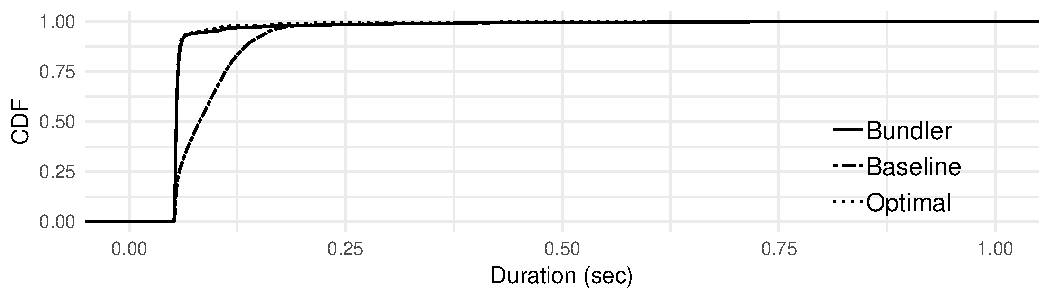
\includegraphics[width=\maxwidth]{figure/eval:best-1} 

\end{knitrout}
    \caption{\name achieves $33$\% lower median slowdown. Note the differing axis scales. For both \name and Optimal, performance benefits come from preventing short flows from queueing behind long ones. \an{Whiskers currently show 1.25 inter-quantile range, figure out how to show 99th \%ile? Also, can barely see Bundler and Optimal...}}
    \label{fig:eval:best}
\end{figure}

\newcommand{\baseline}{Status Quo\xspace}
\newcommand{\optimal}{In-Network\xspace}

\Para{Using \name for fair queueing}
In this section, we evaluate the benefits provided by doing fair queuing at the \name, and use median slowdown as our metric, where the ``slowdown'' of a request is its completion time divided by what its completion time would have been in an unloaded network. A slowdown of $1$ is optimal, and lower numbers represent better performance.

We evaluate three configurations: 
(i) The ``\baseline'' configuration represents the status quo: the \inbox simply forwards packets as it receives them, and the mahimahi bottleneck uses FIFO scheduling.
(ii) The ``\optimal'' configuration deploys fair queueing
at the mahimahi bottleneck.\footnote{
We implement this scheme by modifying mahimahi (our patch comprises $171$ lines of C++) to add a packet-level fair-queueing scheduler to the bottleneck link.}
Recall from \S\ref{s:intro} that this configuration is not deployable.
%: it would force all customers --- who may desire diverging scheduling policies --- to use the same scheduler.
(iii) The default \name configuration, that uses stochastic fair queueing~\cite{sfq} scheduling policy at the \inbox, and (iv) Using \name with FIFO (without exploiting scheduling opportunity).
%\radhika{flip the order for in-network and \name in the figure to be consistent with the above order.}

Figure~\ref{fig:eval:best} presents our results. 
The median slowdown (across all flow sizes) decreases from \overviewBenefitsBaselineMedian 
for Baseline to \overviewBenefitsBundlerMedian 
with \name, \overviewBenefitsBundlerMedianImprovement
lower. 
\optimal's median slowdown is a further 15\% lower then \name: \overviewBenefitsOptimalMedian.
Meanwhile, in the tail, \name's $99\%$ile slowdown is \overviewBenefitsBundlerTail, which is 48\% lower than the \baseline's \overviewBenefitsBaselineTail. \optimal's $99\%$ile slowdown is \overviewBenefitsOptimalTail.

\paragrapha{Using \name for other policies} We additionally evaluated other scheduling and queue management policies with \name. We omit detailed results for brevity, and present a few highlights. With FQ-CoDel~\cite{fq-codel}, \name can achieve 97\% lower median end-to-end RTTs and 89\% lower 99\%ile RTTs.  By strictly prioritizing one traffic class over another, \name results in 65\% lower median FCTs for the higher-priority class. 

\cut{
\subsection{Applying Different Scheduling Policies}\label{s:eval:policies}
%Per \S\ref{s:impl}, our \name implementation can implement any scheduling discipline available in Linux. 

\an{Reduce this subsection to ~one paragraph and roll into 7.2}

In addition to improving FCTs, \name can achieve low packet delay, perform strict prioritization, and rate fairness.

\paragrapha{Achieving Improved Flow Completion Times} \S\ref{s:eval:fct} shows how enabling SFQ at the \name improves the median slowdown by \overviewBenefitsBundlerMedianImprovement.

\paragrapha{Achieving Low Packet Delays}
We enable CoDel~\cite{fq-codel} at the \inbox to lower the packet delays, and test it for a single large backlogged flow using the setup described in \S\ref{s:eval}.
CoDel adds ECN marks to packets in fair-queue buckets which exceed a queue length threshold. 
As a result, endhosts cut their windows earlier, thus reducing their self-inflicted delay within their fair-queue bucket.
We measure the resulting distribution of RTTs seen by the endhost connections with \name and \baseline in Table~\ref{t:eval:codel}.
\begin{figure}
    \centering
\begin{knitrout}
\definecolor{shadecolor}{rgb}{0.969, 0.969, 0.969}\color{fgcolor}
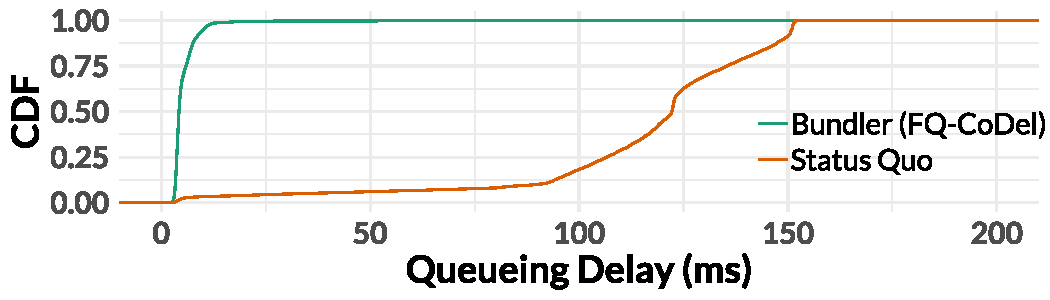
\includegraphics[width=\maxwidth]{figure/eval:lowdelays-1} 

\end{knitrout}
    \caption{We configure \name with the fq-codel scheduling policy to achieve low end-to-end queueing delays.}
    \label{fig:eval:lowdelays}
\end{figure}

As is expected from CoDel, \name in this experiment, achieves \delaysImprovement lower median packet delay than \baseline.

\paragrapha{Strict Prioritization}\label{s:eval:strictprio}
We uniformly divide the web request distribution described in \S\ref{s:eval:setup} into two equally sized classes, one of which is given a higher priority over the other. 
%\radhika{what's the division ratio?}\an{specified equal ratio}  
The results are presented in Table~\ref{t:eval:prio}.
%of traffic transitting \name over a lower-priority class. 

\begin{table}[h]
\begin{center}
\begin{tabular}{c|c|c}
Scheme     &  Median Slowdown                           &  $99$\%ile Slowdown                        \\
\hline
Bundler (Prio.)   &  1.07 &  10.52  \\
Bundler (SFQ)     &  \overviewBenefitsBundlerMedian  &  \overviewBenefitsBundlerTail  \\
\baseline  &  3.07  &  201.72
    \label{fig:eval:strict-prio}
\end{tabular}
\end{center}
\caption{Using strict prioritization further reduces FCTs for the higher-priority class of traffic.}\label{t:eval:prio}
\end{table}
\newcommand{\strictPrioTailImprovementOverFq}{47\%\xspace}
\newcommand{\strictPrioImprovement}{65\%\xspace}


Using a priority scheduler (we use the \texttt{pfifo\_fast} qdisc) at \inbox improves the flow completion times for the higher-priority class compared to \baseline.
Furthermore, prioritization achieves \strictPrioTailImprovementOverFq lower $99$\%ile FCT for the higher priority traffic class, when compared to using fair queueing.

\begin{figure}
    \centering
\begin{knitrout}
\definecolor{shadecolor}{rgb}{0.969, 0.969, 0.969}\color{fgcolor}
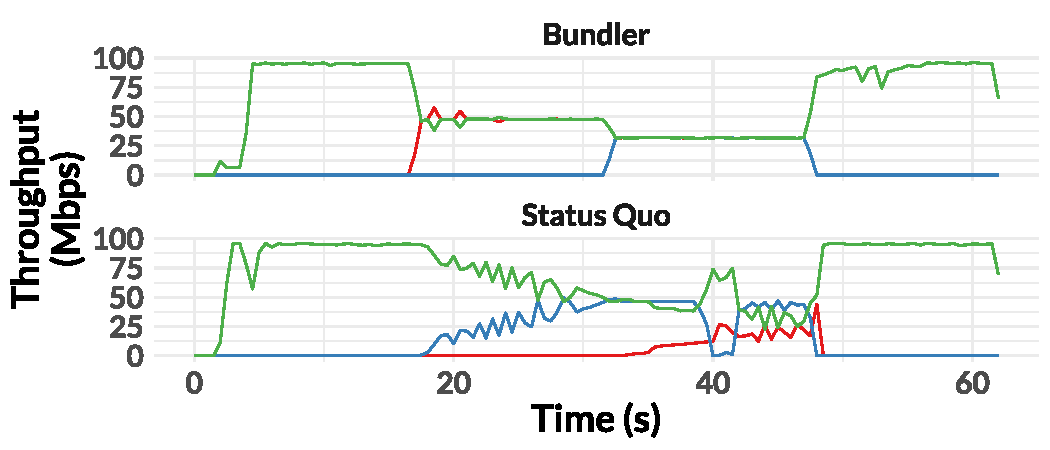
\includegraphics[width=\maxwidth]{figure/eval_waterfall-1} 

\end{knitrout}
    \caption{\name with SFQ achieves fair and stable rates.}
    \label{fig:eval:waterfall}
\end{figure}

\paragrapha{Rate Fairness and Stability}\label{s:eval:waterfall}
We next use our default SFQ scheduler to achieve fairness and rate stability. We start three backlogged flows at different times (0s, 15s, and 30s). Figure~\ref{fig:eval:waterfall} shows that \name converges to fair and stable rates faster than the \baseline.

\begin{figure}
    \label{fig:eval:video}
    \centering
    \begin{subfigure}[b]{0.5\textwidth}
        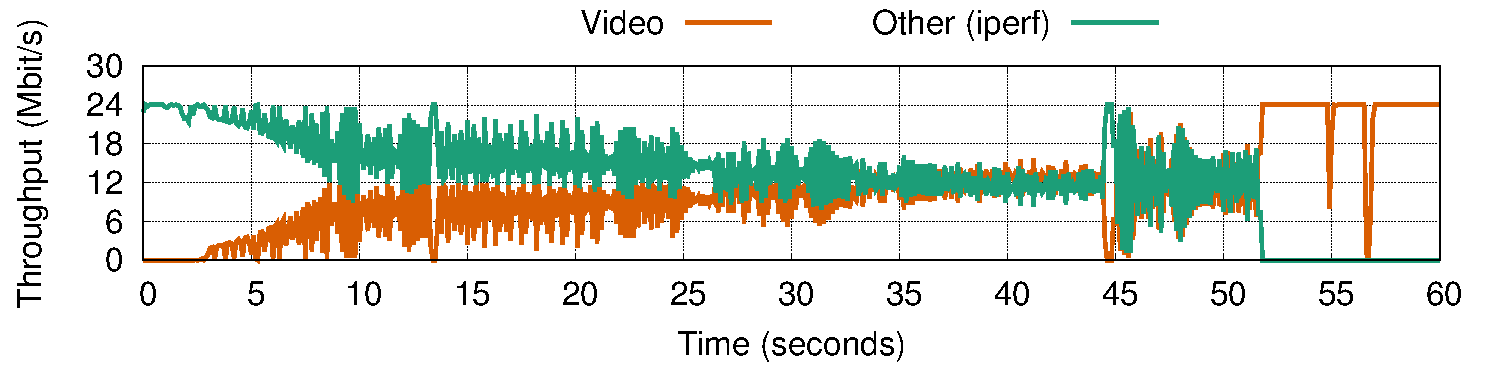
\includegraphics[width=\textwidth]{figure/nobundle-4k-video}
        \caption{Without \name}\label{fig:eval:video:nobundle}
    \end{subfigure}
    \begin{subfigure}[b]{0.5\textwidth}
        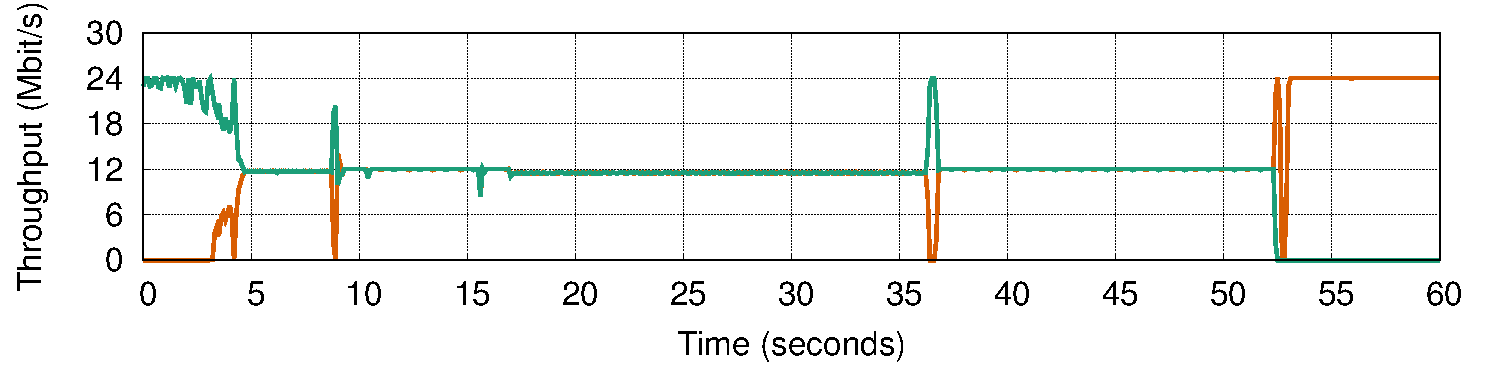
\includegraphics[width=\textwidth]{figure/bundle-4k-video}
        \caption{With \name}\label{fig:eval:video:bundle}
    \end{subfigure}
    \caption{Without \name, the video traffic experiences highly variable throughput, which prevents the ABR algorithm from realizing it could sustain a higher bitrate. \name helps the video flow to quickly converge to the fair rate and stay there, which allows the ABR algorithm to choose the maximum sustainable bitrate.}
\end{figure}

\paragrapha{Rate Stability}\label{s:eval:ratestable}
\fc{come back to this}
In Figure~\ref{fig:eval:video}, we run a persistently backlogged flow over a 24Mbps link and then
after 3 seconds start a client attempting to stream a 4k video from a server that supports adaptive
bitrate selection. Without \name (a), the video stream experiences highly variable throughput and 
takes 30 seconds to converge to a fair share of the link. In contrast, with \name (b), the video
stream converges to its fair share within 2 seconds and is able to maintain that rate for the
entirety of the stream. This stability provides the best scenario for the ABR algorithm to select
the highest possible bitrate and thus maximize QoE.
}

\paragrapha{Aggregate congestion control is not enough} It is important to note that \name's congestion control by itself (\ie running FIFO scheduling) is not a means of achieving improved performance. 
To see why this is the case, recall that \name does not modify the endhosts: they continue to run the default Cubic congestion controller, which will probe for bandwidth until it observes loss.
Indeed, the packets endhost Cubic sends beyond those that the link can transmit must queue somewhere in the network or get dropped. 
Without \name, they queue at the bottleneck link;
with \name, they instead queue at the \inbox. 
In addition, the delay-based congestion controller at \inbox also maintains a small standing queue at the bottleneck link (which can be seen in Figure~\ref{fig:design:shift-bottleneck}) to avoid under-utilization, which increases the end-to-end-delays slightly. 
Therefore, doing the FIFO scheduling at the \name, as is done by the \baseline, results in slightly worse performance.

% cut, combine with overview-benefits
%\begin{figure}
    \centering
\begin{knitrout}
\definecolor{shadecolor}{rgb}{0.969, 0.969, 0.969}\color{fgcolor}
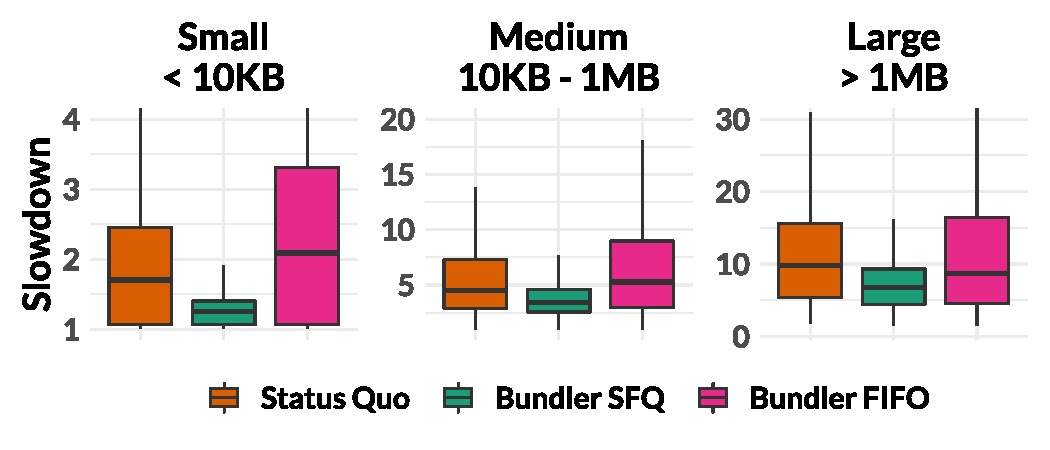
\includegraphics[width=\maxwidth]{figure/eval_fifo-1} 

\end{knitrout}
    \caption{With FIFO scheduling, the benefits of \name are lost: FCTs are 31\% worse in the median. Note the different y-axis scales for each group of request sizes.}
    \label{fig:eval:fifo}
\end{figure}
\newcommand{\overviewBenefitsFifoMedian}{2.13\xspace}
\newcommand{\overviewBenefitsFifoWorse}{31\%\xspace}


\subsection{Impact of Cross Traffic}\label{s:robust:cross}


\newcommand{\bigexpBundlerElasticSlowdown}{2.6251566\%\xspace}
\newcommand{\bigexpNoBundlerElasticSlowdown}{2.3453956\%\xspace}
\newcommand{\bigexpElasticSlowdownWorseness}{12\%\xspace}

\begin{figure*}
\begin{centering}
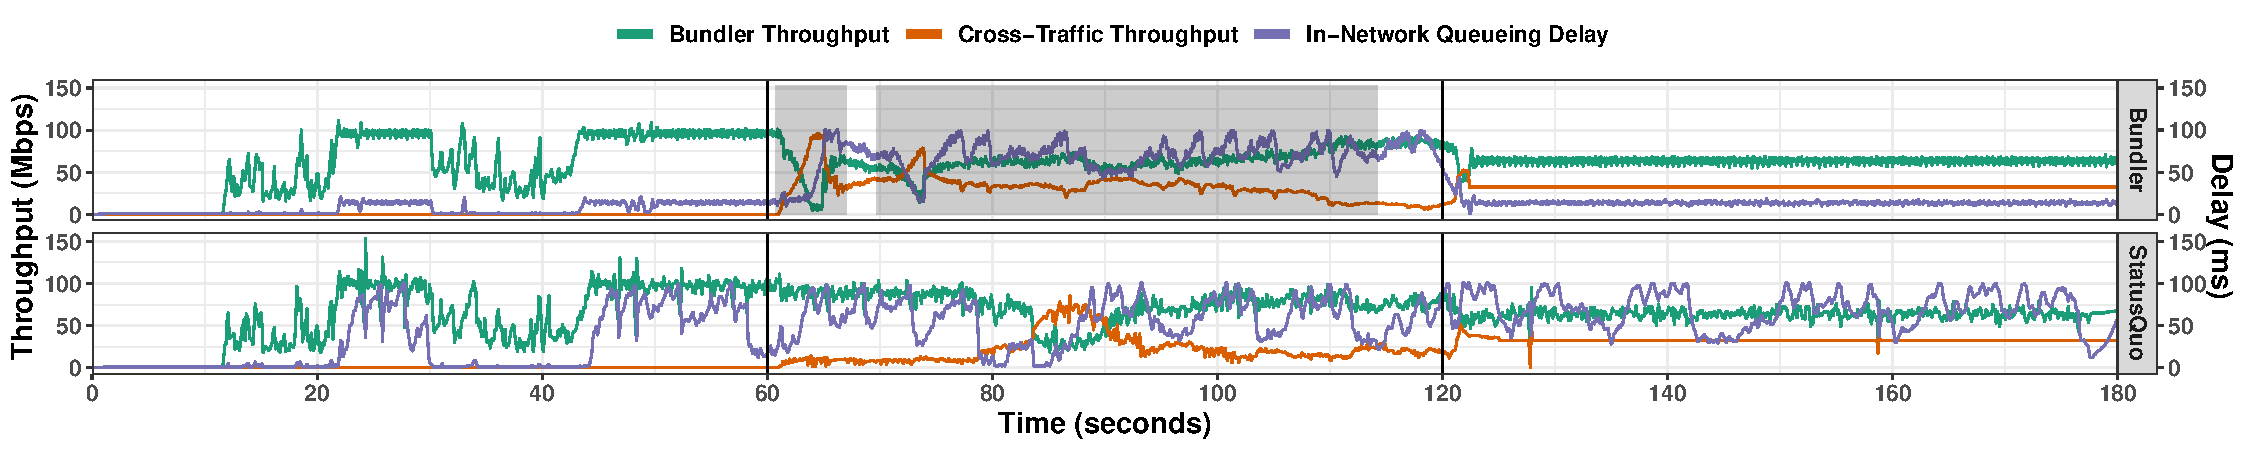
\includegraphics[width=\textwidth]{big_exp/timeseries}
\end{centering}
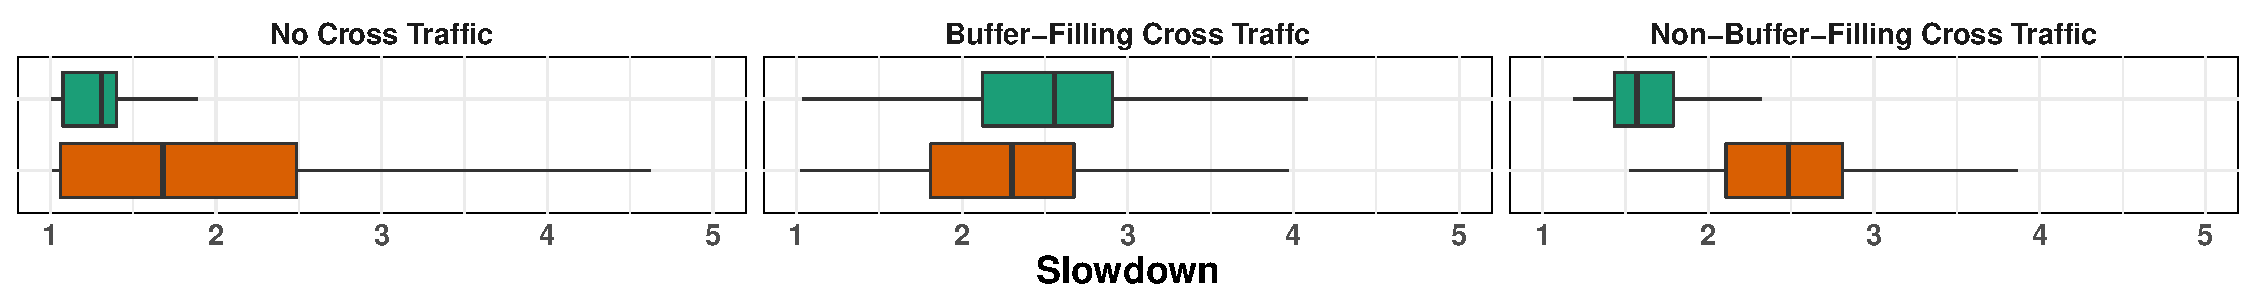
\includegraphics[width=0.95\textwidth]{big_exp/fcts}
\caption{\name's scheduling ability depends on the characteristics of the cross traffic over time. In this experiment, there are 3 periods: from 0 to 60 sec., there is no competing traffic, from 60 to 120 sec. there is buffer-filling cross traffic, and from 120 to 180 sec. there is non-buffer-filling cross traffic. The box-plots below each period show the distribution of short flow FCTs during that time. During the period with buffer-filling cross traffic, \name detects its presence and competes fairly. The shaded region indicates time \name spent in buffer-filling cross-traffic mode (\Sec{s:buffer-filling}).}\label{fig:eval:bigexp}
\end{figure*}

Can \name successfully revert to status-quo performance in the presence of buffer-filling cross traffic, then resume providing benefits once that cross traffic leaves?
In Figure~\ref{fig:eval:bigexp}, we show this scenario.
At first, the link is occupied only by \name's traffic, similar to the setup described in \S\ref{s:eval:setup}.
At time $t=60$~sec, a buffer-filling cross traffic flow arrives.
\name detects its presence (indicated by the gray shading) and starts pushing more packets into the network to compete fairly, reverting back to performance that is slightly worse than Status Quo (median FCT for short flows is \bigexpElasticSlowdownWorseness higher). 
Performance is slightly worse because of the $10$ms queue that \name continues to maintain at its \inbox for active probing to detect the cross-traffic's departure, as described in \S\ref{s:queue-ctl}.
\footnote{We believe the benefits provided by \name in the more common regime with no competing buffer-filling cross traffic are substantial enough to make up for slight degradation in these specific scenarios.}
At time $t=120$sec, the buffer-filling flow stops and non-buffer-filling traffic starts, generated from the same distribution as \name as described in \S\ref{s:eval:setup}.
\name correctly detects that it is safe to resume delay-control, and continues providing scheduling benefits.
For the remainder of this subsection, we present three micro-benchmarks which dig deeper into the latter two scenarios, where cross traffic can affect \name's performance. 
We present results with both Nimbus and Copa being used as the congestion control algorithm at the \inbox. 
\cut{In \S\ref{s:eval:offeredload} we present further results on how well \name retains benefits with varying amounts of offered load.}

\begin{figure}
    \centering
\begin{knitrout}
\definecolor{shadecolor}{rgb}{0.969, 0.969, 0.969}\color{fgcolor}
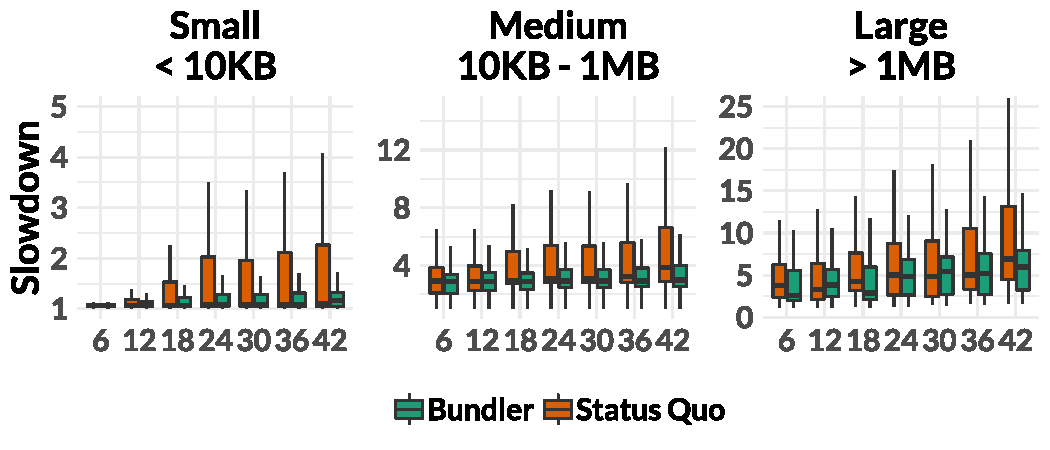
\includegraphics[width=\maxwidth]{figure/robust_cr-inelastic-1} 

\end{knitrout}
    \caption{Against cross traffic comprising of short lived flows. \name offers 48Mbps of load to the bottleneck queue. The cross traffic's offered load increases along the x-axis, while \name{}'s offered load remains fixed.}
    \label{fig:robust:cr-inelastic}
\end{figure}

\paragrapha{Mix of flow sizes} 
We first consider in Figure~\ref{fig:robust:cr-inelastic} the case \name traffic is most likely to encounter, where the cross traffic comprises of finite-length flows up to a few MBs.
We draw both \name's traffic and the cross traffic from the same measured distribution of web requests described in \S\ref{s:eval:setup}.
We fix \name's offered load at a constant $48$ Mbit/s and vary the cross traffic's offered load from $6$ to $42$ Mbit/s.

While flows are often short, they sometimes exit slow start. With sufficient offered load, they can cause queueing in the aggregate. 
Observe that the \baseline FCTs increase steadily as the cross traffic's offered load increases: this is due to the aggregate queueing effect.
When this happens, Bundler responds by temporarily reducing its sending rate to lower the delay, because the cross traffic has not been deemed elastic. 
Importantly, this rate reduction is short-lived because these cross-traffic flows are short-lived, and long-term Bundler throughput is not reduced.
We believe that this trade-off (short-term throughput reduction for better delay) is a good one. 
The lower delay helps the short flows in the bundle, while the large flows in the bundle are not affected by the short-term throughput reduction. 
``Mid-sized'' flows in the bundle can be affected if \name sacrifices throughput for too long. 
By design, however, \name detects such cross-traffic and disables its delay-control mechanism in response.

\begin{figure}
    \centering
    \begin{subfigure}[b]{0.5\textwidth}
\begin{knitrout}
\definecolor{shadecolor}{rgb}{0.969, 0.969, 0.969}\color{fgcolor}
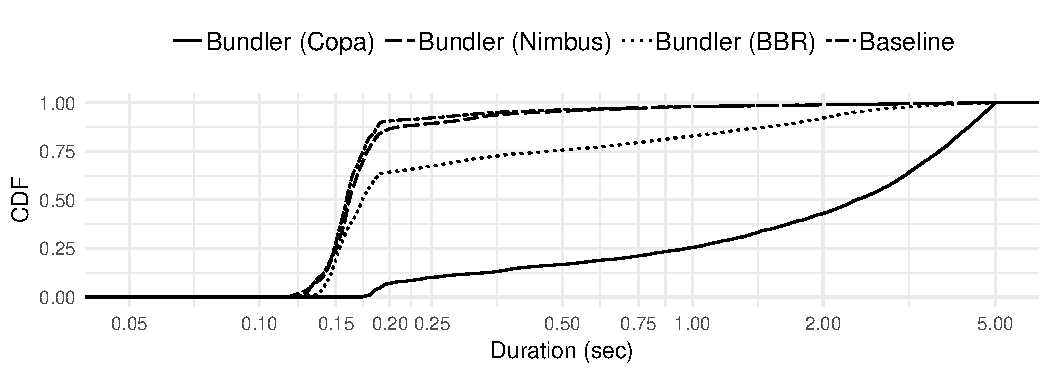
\includegraphics[width=\maxwidth]{figure/robust:cr-elastic:a-1} 

\end{knitrout}
    \caption{Congestion controllers from \S\ref{s:eval}.}\label{fig:robust:cr-elastic:a}
    \end{subfigure}
    \begin{subfigure}[b]{0.5\textwidth}
\begin{knitrout}
\definecolor{shadecolor}{rgb}{0.969, 0.969, 0.969}\color{fgcolor}
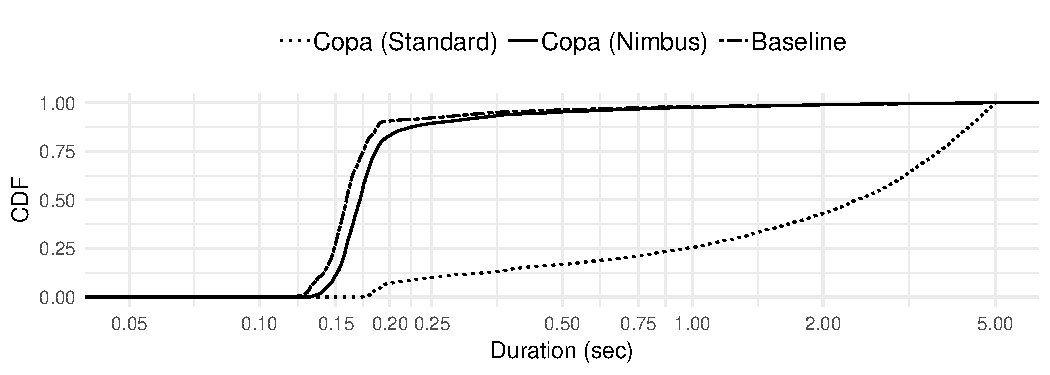
\includegraphics[width=\maxwidth]{figure/robust:cr-elastic:b-1} 

\end{knitrout}
    \caption{Alternate configuration -- Copa uses Nimbus's elasticity detector.}\label{fig:robust:cr-elastic:b}
    \end{subfigure}

    \caption{Elastic cross traffic.}
    \label{fig:robust:cr-elastic}
\end{figure}

\paragrapha{Persistent elastic flows} 
We now evaluate how \name's throughput is impacted due to competition from varying amounts of persistent elastic cross-traffic. 
As discussed in \S\ref{s:queue-ctl}, we believe this synthetic scenario is rare in practice, but when it does occur, \name cannot provide benefits, and since it must ``hold back'' some queue to detect when the cross-traffic subsides, its traffic will experience RTT inflation.
Indeed, Figure~\ref{fig:robust:cr-elastic} shows that 
the component flows in the bundle experience  \bundlerElasticTputWorseness less throughput on average. 
The impact varies from \bundlerElasticTputWorsenessTen lower throughput with 10 competing flows to \bundlerElasticTputWorsenessFifty lower with 50. 

\begin{figure}
    \centering
\begin{knitrout}
\definecolor{shadecolor}{rgb}{0.969, 0.969, 0.969}\color{fgcolor}
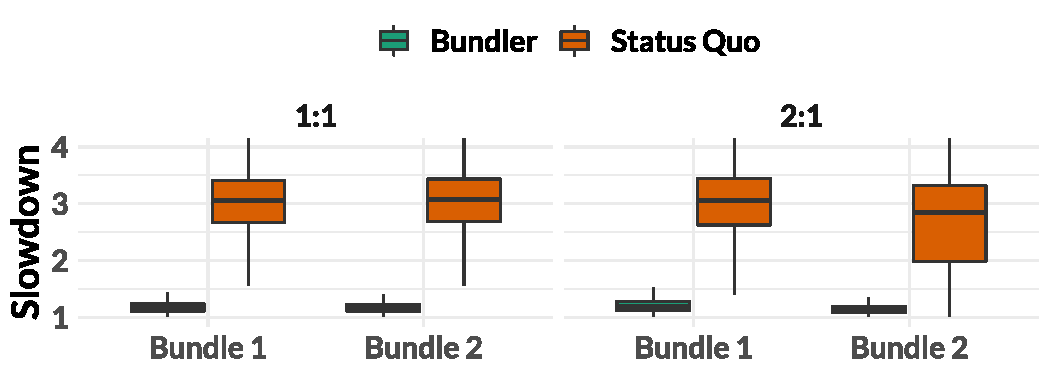
\includegraphics[width=\maxwidth]{figure/robust_twobundler-1} 

\end{knitrout}
    \caption{Competing traffic bundles. In both cases, the aggregate offered load is 84Mbps, as in Figure~\ref{fig:eval:best}. For "1:1", we evenly split the offered load between the two Bundles; for "2:1", one bundle has twice the offered load of the other. In both cases, each bundle observes improved median FCT compared to its performance in the baseline scenario.}
    \label{fig:robust:twobundler}
\end{figure}

\paragrapha{Competing Bundles} Last, we evaluate the case where flows from multiple bundles compete with one another. 
In Figure~\ref{fig:robust:twobundler}, we show the performance with two bundles of traffic competing with one another at the same bottleneck link. 
Both bundles comprise of web requests along with a backlogged Cubic flow. 
%Even in the presence of this buffer-filling cross traffic, 
%\radhika{??? i believe the backlog flow is in the bundles and not outside it}
%\an{yes, it is, that's why the perf is good. I agree we should reword, it is confusing}
Both bundles maintain low queueing in the network and successfully control the queues at the \inbox.
Thus, \name provides benefits for both bundles, even when the amount of traffic in each bundle is different.  

\subsection{Impact of Congestion Control}\label{s:eval:cc}

%\an{I have cut down this subsection: removed the e2e congestion control figure and replaced with inline text}
We now evaluate the impact of a different congestion control algorithm running at the \inbox and at the endhosts.

\begin{figure}
    \centering
\begin{knitrout}
\definecolor{shadecolor}{rgb}{0.969, 0.969, 0.969}\color{fgcolor}
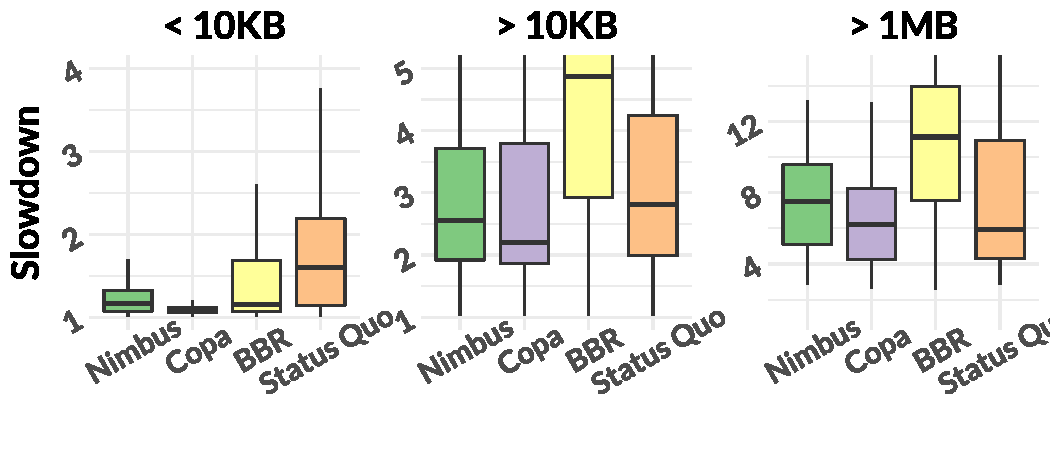
\includegraphics[width=\maxwidth]{figure/eval:cc-1} 

\end{knitrout}
    \caption{Choosing a congestion control algorithm at \name remains important, just as it is at the end-host. Note the different y-axis scales for each group of request sizes.}
    \label{fig:eval:cc}
\end{figure}
\newcommand{\ccCopaMedian}{}
\newcommand{\ccNimbusMedian}{}
\newcommand{\ccBBRMedian}{}
\newcommand{\ccBaselineMedian}{}


\Para{\capinbox congestion control} So far we have evaluated \name by running Copa~\cite{copa} at the \inbox. 
Figure~\ref{fig:eval:cc} shows \name's performance with other congestion control algorithms (namely, Nimbus's BasicDelay~\cite{nimbus-arxiv} and BBR~\cite{bbr}), and using SFQ scheduling. 
We find that using BasicDelay provides similar benefits over \baseline as Copa. 
BBR, on the other hand, performs slightly worse than \baseline. 
This is because it pushes packets into the network more aggressively than the other schemes, resulting in a bigger in-network queue.
This, combined with the queue built at the \name, results in the endhosts experiencing higher queueing delays than \baseline. This shows that the choice of congestion control algorithm, and its ability to maintain small queues in the network, plays an important role. 

\Para{Endhost congestion control} We used Cubic congestion control at the endhosts for our experiments so far. When we configure endhosts to use Reno or BBR, \name's benefits remain: \name achieves 58\% lower FCTs in the median compared to the updated \baseline where the endhosts use BBR. 
This shows that \name is compatible with multiple endhost congestion control algorithms.
%This is primarily because in the \baseline, using BBR causes endhosts to achieve 66\% worse median slowdown ($1.62$ with Cubic to $2.68$ with BBR); \name's slowdown is only 5\% worse when endhosts use BBR ($1.08$ with Cubic to $1.14$ with BBR). 

\cut{
\begin{figure}
    \centering
\begin{knitrout}
\definecolor{shadecolor}{rgb}{0.969, 0.969, 0.969}\color{fgcolor}

\includegraphics[width=\maxwidth]{figure/eval_e2e-1} 

\end{knitrout}
    \caption{\name still provides benefits when the endhosts use different congestion control algorithms.}
    \label{fig:eval:traffic}
\end{figure}

\Para{Endhost congestion control} 
We used Cubic congestion control at the endhosts for our experiments so far. When we configure endhosts to use Reno or BBR (as implemented in Linux $4.13$), \name's benefits remain (Figure~\ref{fig:eval:traffic}).
%: in Figure~\ref{fig:eval:traffic}, \name achieves 58\% lower FCTs in the median compared to the updated \baseline where the endhosts use BBR. 
%This is primarily because in the \baseline using BBR causes endhosts to achieve 66\% worse median slowdown ($1.62$ with Cubic to $2.68$ with BBR); \name's slowdown is only 5\% worse when endhosts use BBR ($1.08$ with Cubic to $1.14$ with BBR). 
This shows that \name is compatible with multiple endhost congestion control algorithms.
}


\cut{
\begin{Appendix}
\section{Varying Offered Load}\label{s:eval:offeredload}
Naturally, if a link is less congested, scheduling the packets that traverse it will have less benefit. Accordingly, as the offered load is reduced, we would expect the gains from scheduling to diminish. 
We now use the web request distribution described in \S\ref{s:eval:setup} to generate a load of 50\% ($48$Mbps), 75\% ($72$Mbps) and 87.5\% ($84$Mbps) of the bottleneck link bandwidth. Our results in Figure~\ref{fig:eval:offeredload} show that as the offered load is decreased, the benefits of \name reduce. This is because if a link is less congested, scheduling the packets that traverse it will have less benefit.
% At 87.5\% load, even without the load offered by a persistently backlogged connection, \name improves FCTs by \an{amount}. 
% As the offered load decreases to 50\%, the benefit provided by \name decreases as well -- to \an{amount} at the 75th percentile.
\end{Appendix}
}

\subsection{Terminating TCP Connections}\label{s:eval:proxy}

Although our \name prototype does not terminate connections (as discussed in \S\ref{s:design:whichcc}), we note that terminating connections does provide one key advantage: the end-to-end congestion controller will observe a smaller RTT, since the proxy can acknowledge its segments much faster than the original receiver. 
This enables rapid window growth at the endhosts.
While there are, of course, operational concerns with managing the resulting queue, it does provide additional scheduling opportunities as well as faster ramp-up for midsized connections.

How much benefit, then, could a proxy-based \name provide?
To evaluate this, we emulate an idealized TCP proxy by modifying the endhosts to maintain a constant congestion window of $450$ packets---slightly larger than the bandwidth-delay product in our setup---and increasing the buffering at the \inbox to hold these packets. 
The other aspects of \name remain unchanged.
The result is in Figure~\ref{fig:eval:proxy}. 

For the short requests which never leave TCP slow start, terminating TCP connections does not yield additional benefits: with or without termination, they finish in a few RTTs.
For medium-to-long requests, terminating TCP connections yields additional benefits since they no longer incur the penalty of window growth.
Therefore, a site may benefit from proxying TCP connections at \name if its traffic pattern contains many medium-sized flows which benefit from fast ramp-up.

\begin{figure}
    \centering
\begin{knitrout}
\definecolor{shadecolor}{rgb}{0.969, 0.969, 0.969}\color{fgcolor}
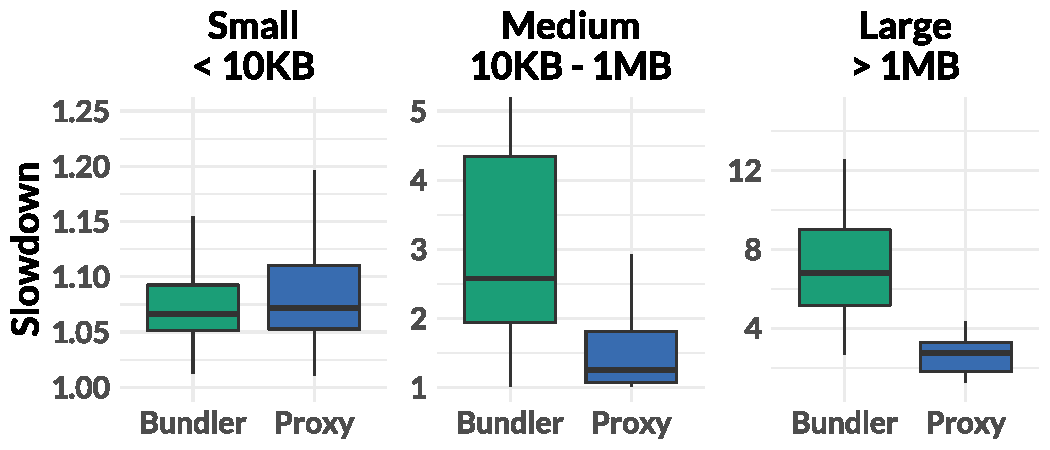
\includegraphics[width=\maxwidth]{figure/eval_proxy-1} 

\end{knitrout}
    \caption{A proxy-based implementation of \name could yield further benefits to the long flows. Note the different y-axis scales for each group of request sizes.}
    \label{fig:eval:proxy}
\end{figure}


\subsection{Multipath Detection}\label{s:eval:ecmp}

% TODO: after deadline should also run experiment where there are > 1 queues but no imbalance, and then suddenly a large flow comes in and creates imbalance, then leaves, heuristic should go above threshold and come back down correspondingly 
As described in \S\ref{s:queue-ctl:ecmp}, when the ratio of out-of-order to in-order measurements is above a certain threshold, it indicates that \name's component flows are likely traversing multiple imbalanced paths. To evaluate the extent to which this heuristic corresponds with imbalance, we re-run the emulation experiment from Figure~\ref{fig:eval:bigexp} for a variety of network conditions (bottleneck bandwidth ranging from 12 to 96 Mbps, end-to-end RTTs ranging from 10 to 300 ms, and bottleneck load-balancing from 1 to 32 paths) and consider the average value reported by the heuristic over each experiment. The maximum value reported across all experiments with a single path was 0.4\%, while the minimum value reported across all experiments with 2-32 paths was 20\%, two orders of magnitude greater. Thus, this heuristic provides a very clear separation between single and multiple path scenarios and a simple threshold is sufficient. 

% Motivated by these results, we use 0.05 as a threshold for our real-world experiments in the following section. We classified each path as single or multipath by whether or not the component flows experienced different min-RTTs (which we can do in this experiment since we control the flows but \name would not be able to do itself), and found that our chosen threshold correctly distinguished between single and multiple path in all cases. 

% \begin{figure}
%     \centering
% 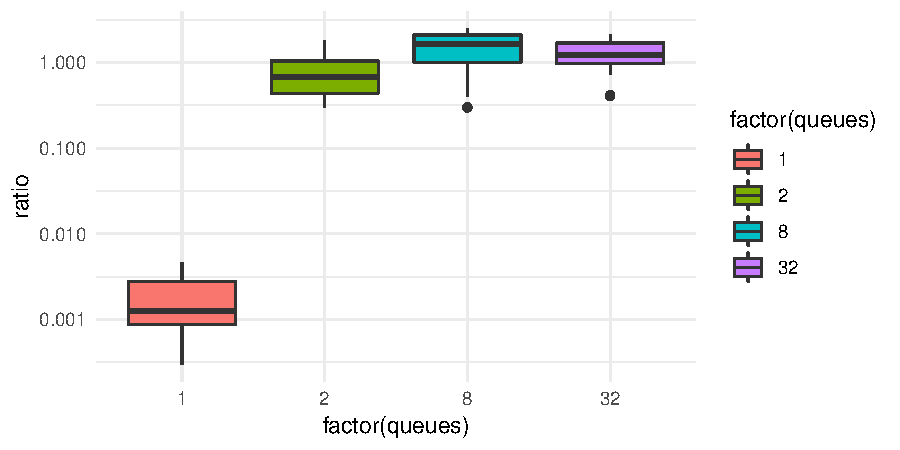
\includegraphics[width=\maxwidth]{figure/eval:ecmp:ratio} 
%     \caption{The queue imbalance heuristic as a function of number of queues. }
%     \label{fig:eval:ecmp:ratio}
% \end{figure}

\section{Real Internet Paths}\label{s:eval:realworld}

\cut{
\begin{outline}
\1 Thus far, we have developed our system under the assumption of a single bottleneck.
\1 We now turn to answer two questions:
    \2 How prevalent is multi-pathing in the Internet?
    \2 How does \name handle multi-pathing?
\1 To answer question (1), we conduct a measurement study from various datacenters to randomly selected IPv4 addresses.
    \2 We used Scamper~\cite{scamper} in ``trace-lb'' mode, which varies the source port of outgoing UDP packets while limiting their TTL, to observe traceroute-style responses from the various paths along the route to the destination.
    \2 We studied \an{XXX} source AWS and Azure datacenters and \an{YYY} random destination IPv4 addresses across \an{ZZZ} unique destination ASes.
    \2 We observe no IP-level multipathing on \an{XXX}\% of paths. The remainder of paths had at least one instance of IP-level multipathing, that is, two UDP packets with the same TTL received TTL-exceeded responses from different source IPs.
    \2 In these cases, we considered the type of multipathing that occurred. If the path between two ASes is load-balanced between two or more intermediate ASes, we cannot really consider the path an aggregate because congestion conditions between the two intermediate ASes may be different.
        \3 However, if there is no AS-level load balancing, then local load balancing is a tractable problem to solve. \an{why}
    \2 In our experiments there were \an{XXX} cases of AS-level multipathing. Further, in cases where there was multipathing, the component routers in the load-balanced hop had similar RTTs.
\end{outline}
}

\begin{figure}
    \centering
\begin{knitrout}
\definecolor{shadecolor}{rgb}{0.969, 0.969, 0.969}\color{fgcolor}
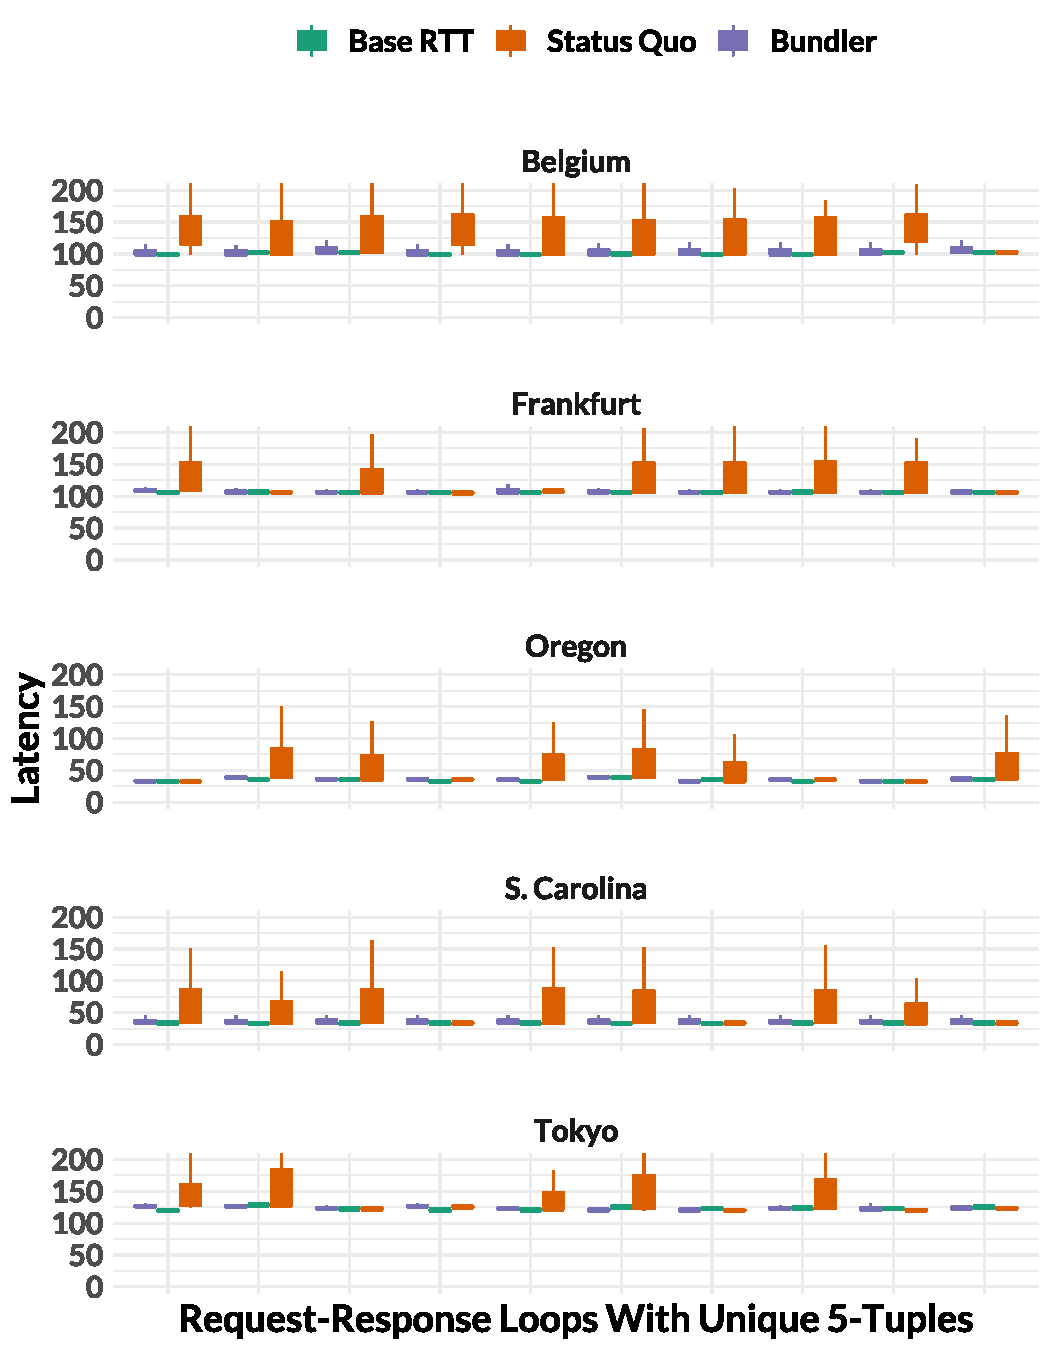
\includegraphics[width=\maxwidth]{figure/eval:realworld-1} 

\end{knitrout}
    \caption{On 5 real-Internet paths from the GCP datacenter in Iowa, \name achieves close to the Base RTT for latency-sensitive traffic. Each bar depicts an individual 5-tuple. On some paths, load-balancing in the Internet causes only some 5-tuples to experience queueing. \name offers scheduling for those paths.}
    \label{fig:eval:realworld}
\end{figure}
%\newcommand{\overviewBenefitsBundlerMedianImprovement}{round(100*(1-(overview_benefits_bundler_results[1] / overview_benefits_baseline_results[1])), 0)\%\xspace}

We next evaluate our prototype implementation on real Internet paths to demonstrate that \name can effectively shift queues in practical settings.
% We next evaluate our prototype implementation on real Internet paths to answer three key questions that our emulated setup did not answer: (1) Does congestion (and queuing) actually occur in the middle of the network? (2) Is buffer-filling cross traffic rare enough in practice to ensure that \name provides a net improvement in performance? and (3) Is \name's design robust to possible multi-pathing effects in a real network? Our results reveal an affirmative answer for all three questions. We explain our experiment setup and results below. 

\Para{Experiment Setup} 
We deploy \name (\inbox) in a GCP datacenter in Iowa and generate traffic from multiple different machines in this datacenter (as detailed below). 
The generated traffic is sent to multiple machines in five different GCP datacenters (in Belgium, Frankfurt, Oregon, South Carolina, and Tokyo). We configured GCP to route traffic over the public Internet rather than a private network. 
We deploy a \name (\outbox) in each of these receiving datacenters, thus resulting in a total of five bundles spanning different regions of the globe.

We evaluate two different workloads in this setup: (i) Each bundle comprising of 10 parallel closed-loop 40 bytes UDP requests, where the sender issues a new request every time it receives a response. We measure the request-response RTTs in this workload to use as a baseline (and call them Base RTTs). (ii) We add 20 backlogged (\texttt{iperf}) flows to the above workload in each bundle. We run this workload both with and without \name and measure the UDP request-response RTTs (represented as \name and \baseline respectively). Effective SFQ across all flows with \name should not inflate the base request-response RTT.
We verified that the backlogged senders achieve similar throughput in all cases (2-4Gbit/s on these paths) both with and without \name, and that the \name machine in Iowa is not a bottleneck itself. 

\Para{Result} 
Figure~\ref{fig:eval:realworld} shows, for each of the five bundles, the resulting RTT distributions for each of the ten request-response loops (with the 5 tuples in UDP/IP headers differing across all ten). 
We make two key observations: (i) The \baseline RTTs are significantly higher than the Base RTT, which indicates significant queueing outside of either site's control. (ii) \name is able to move these queues and enforce SFQ scheduling effectively, resulting in request-response RTTs comparable to Base RTTs, and \realworldMedianLatencyImprovement smaller than \baseline at the median.
% (iii) The \baseline results further reveal that different request-response loops within a given bundle see different amounts of queueing in the network. This indicates possible ECMP load-balancing in the network based on the 5 tuples, and how \name is robust to its effects.

\Para{Explanation}
Observation (i) above indicates that all of the conditions in \S\ref{s:deploy} held during our experiment and that queues were indeed building outside of our control. 
One possibility is that these queues built up at an egress rate limiter imposed by GCP. 
However, our throughput measurements suggest that this is unlikely\footnote{We lack visibility into Google's network and thus were unable to determine the true location of the bottleneck in this experiment.}; we used \texttt{n1-standard-2} machines, which have a maximum possible egress of 10Gbps each, but our backlogged senders achieved only 2-4Gbps. 
Nevertheless, even if queues did form at GCP's rate limiter, this represents a scenario where \name is useful: 
an operator deploying an application between multiple cloud regions could use \name to enforce scheduling policies on their traffic without negotiating their policy with the cloud provider or knowing where the bottleneck occurs. 

\section{Discussion}\label{s:discussion}

\paragrapha{Composability} Bundles are naturally \emph{composable}: a sub-site within site A can deploy its own \name to take control of its fraction of the in-network queues, with the site A's \name enforcing a scheduling policy across the bundled traffic from each sub-site.  
%\radhika{finally at the right place! but needs more exposition.}
%\an{added some exposition below}
For example, a department within an institute may bundle its traffic to a collaborating department in another institute, with the parent institutes bundling the aggregate traffic across multiple departments.
% \name may be useful at \emph{both} levels of aggregation, because different amounts of traffic experience bottlenecks in different locations.
% An individual user could be bottlenecked on a slow Wi-Fi link. 
% This individual's traffic might mix with an institute's department which, as an aggregate, is bottlenecked on the campus's local network.
% After another layer of aggregation, the institute's traffic could be bottlenecked on an interdomain link.
% At each layer of aggregation, it may be beneficial to control the queues at the respective \name.
% Studying this deployment scenario remains future work.

\paragrapha{Scheduling across different bundles at a \inbox} We evaluate benefits of scheduling \emph{within} a bundle. In practice, a given \inbox will see traffic from multiple bundles. Extending different scheduling policies to multiple such bundles can be done trivially.
%Different bundles may have different rates; recent work~\cite{carousel, eifel} has shown it is possible to implement such multi-rate, multi-scheduler datapaths efficiently.

\paragrapha{Rate allocation across different competing bundles} When multiple bundles (belonging to different sites) compete at the same bottleneck, \name's congestion control would ensure a fair rate allocation across each of these bundles, irrespective of the amount of traffic in them. It, therefore, provides fairness on per-site basis, as opposed to a per-flow basis, making it more robust to popular end-host strategies such as opening multiple connections to increase bandwidth share. 

\section{Conclusion}\label{s:concl}
We have described \name, a new type of middlebox which uses a novel ``inner''  congestion control loop for traffic bundles between two sites to shift the queues from the middle of the network, where it is difficult to unilaterally express traffic control policy, to the site itself, where doing so is tractable. 
\name neither maintains any per-flow state, nor makes any modifications to the packets. 
We demonstrate, using both emulated network experiments and real Internet paths, that it is possible to shift queues and schedule packets to an extent sufficient to enforce well-known scheduling disciplines. 

\cut{In our experiments, we used fair queueing to improve median FCTs by \overviewBenefitsBundlerMedianImprovement, strict prioritization to improve $99$\%ile FCTs of a high-priority traffic class by \strictPrioImprovement, and AQM to reduce end-to-end packet delays by \delaysImprovement.}
%\vspace{-5pt}
%\paragrapha{Statement of ethics considerations} This work does not raise any ethical issues.

\label{s:acknowledgements}
\paragrapha{Acknowledgements} We thank xxx.
This work was supported in part by DARPA contract HR001117C0048 and NSF grant 1407470.


\label{p:end}
% \begin{appendix}
\section{Queue Controller Stability}\label{app:derive-ab}

\name{} controls the queues by updating its sending rate according to the following equation:
\begin{equation} 
    \dot{r}(t) = \alpha (q(t) - q_T) + \beta (\dot{q}(t))
\end{equation}
%
How should we set $\alpha$ and $\beta$? This decision is related to the size of the Nimbus pulse. 
If the queue controller is too aggressive (\ie it reacts quickly to maintain the queue target), it will nullify the Nimbus pulse with its overlaid rate control.
If it is too timid, it will not be able to effectively control the queues.

Therefore, we want the target queue length to be $A \sin(\frac{2\pi{}t}{T})$. 
We can write how the queue length varies with time as (where $\mu$ is the link bandwidth):
    \vspace{-5pt}
\begin{equation} 
    \dot{q}(t) = \mu - r(t) - A \sin(\frac{2\pi{}t}{T})
\end{equation}
%
\noindent Thus, 
%
\begin{equation}
    \ddot{q}(t) = - \dot{r}(t) - A \frac{2\pi{}t}{T} \cos(\frac{2\pi{}t}{T})
\end{equation}
%
\noindent Combining with the rate update rule:
%
\begin{equation}
    \ddot{q}(t) - \beta \dot{q}(t) + \alpha (q(t) - q_T) = A \frac{2\pi{}t}{T} \cos(\frac{2\pi{}t}{T})
\end{equation}
%
\noindent Substituting the pulse parameters from Nimbus and using $y(t) = q(t) - q_T$, we write a second-order ordinary differential equation (ODE) with sinusoidal input:
%
\begin{equation}
    \ddot{y}(t) - \beta \dot{y}(t) + \alpha y(t) = 10\pi{}A \cos(10\pi{}t)
\end{equation}
%
\noindent This has the standard-form solution:
%
\begin{equation}
    y(t) = c_1 e^{r_1 t} + c_2 e^{r_2 t} + \frac{10\pi{}A}{|p(10\pi{}i)|} \cos(10\pi{}i - \phi)
\end{equation}
%        
where $p$ is the characteristic polynomial and $r_1, r_2$ are its roots;
\ie 
\begin{equation}
r_1 = \frac{-\beta + \sqrt{\beta^2 - 4\alpha}}{2}, r_2 = \frac{-\beta - \sqrt{\beta^2 - 4\alpha}}{2}
\end{equation}
%
\noindent We want: (1) the $r_1$, $r_2$ to be large, so the queue converges quickly, and (2) the pulse amplitude to be approximately the Nimbus pulse amplitude, so:
%
\begin{equation}
\frac{10\pi{}A}{|p(10\pi{}i)|} \approx \frac{A}{5\pi}
\end{equation}

\noindent $\alpha = 10, \beta = 10$ satisfy these constraints.
\end{appendix}

\end{sloppypar}
\clearpage
\bibliographystyle{abbrv}
\bibliography{ref}
\end{document}
